\documentclass[12pt,a4paper,oneside]{scrbook}
\usepackage{mystyle}

% faster tikz. Needs to be here because of overleaf
\usepgfplotslibrary{external}
\tikzexternalize[prefix=tikzexternalize/]

\makeatletter
\renewcommand{\todo}[2][]{\tikzexternaldisable\@todo[#1]{#2}\tikzexternalenable}
\makeatother


\date{\today}
% \publishers{Universität Stuttgart}

\begin{document}

\tikzexternaldisable
\begin{titlepage}
    \begin{tikzpicture}[overlay,remember picture,y=-1cm]
        % set a new origin [1]
        \coordinate (O) at (current page.north west);
        \draw[fill=white,draw=yellow] ($(O)+(6.51,9.32)$) rectanglenode[align=center]{
                \large Bachelorarbeit
                \\
                \\
                \Large \textbf{Anwendung von}\\
                \Large \textbf{Contraction Hierarchies und} \\
                \Large \textbf{Hierarchical Hub Labeling}\\
                \Large \textbf{auf Nicht-Straßengraphen}
                \\
                \\
                \large Christian Staib
            } ($(O)+(15.37,14.97)$);
    \end{tikzpicture}
\end{titlepage}
\tikzexternalenable

\clearpage

\chapter*{Kurzfassung}
Die Technik der Contraction Hierarchies (CH) und der Hierarchical Hub Labelings (HL) haben sich als äußerst wirksame Techniken zur Beschleunigung von Routenanfragen in Straßennetzwerken erwiesen. Die Anwendung auf Graphen außerhalb des Straßenverkehrs wurde weit weniger untersucht - ein Beispiel hierfür findet sich z.B. in [1] -, auch wenn in diesen Fällen ebenfalls eine schnellere Anfrage von Suchanfragen wünschenswert ist.

Ziel dieser Arbeit ist es, diese Fragestellung eingehender zu untersuchen. Es sind hierbei sowohl andere Graphtypen zu betrachten, als auch ggf. bessere Konstruktionsstrategien für CH bzw. HL zu entwerfen. Graphtypen, die potenziell von Interesse sind:

\begin{itemize}
      \item
            Sichtbarkeitsgraphen
      \item
            Gridgraphen, wie sie z.B. in Computerspielen vorkommen
      \item
            Kommunikationsgraphen
      \item
            Kollaborationsgraphen
      \item
            Linkgraphen (z.B. von Wikipedia)
\end{itemize}
\tableofcontents
\chapter{Einleitung}

\section{Problemstellung}
Sichtbarkeitsgraphen sind Graphen, die alle Knotenpaare miteinander verbinden, die sich \emph{sehen} können, auf deren \emph{Luftlinie} sich also keine \emph{Hindernisse} befinden.
Aus einer Küstenlinie kann ein Sichtbarkeitsgraph erstellt werden, indem die Knoten auf der Küstenlinie mit allen Knoten verbunden werden, deren Luftlinie keine Küste kreuzt.
\autoref{fig:thessaloniki-visibility} zeigt einen Ausschnitt eines solchen Sichtbarkeitsgraphen.
Zu sehen ist der Hafen der griechischen Stadt Thessaloniki.

Das Finden von kürzesten Pfaden ist in solchen Graphen rechenintensiver als etwa auf Straßengraphen mit vergleichbarer Knotenanzahl, da sie unter anderem einen höheren durchschnittlichen Knotengrad und keine inhärente hierarchische Struktur besitzen.
Zwar gibt es Möglichkeiten, den Graphen zu verändern, und schneller Pfade zwischen Knoten zu berechnen, etwa durch Triangulierung oder Rasterisierung, jedoch sind diese Pfade nicht mehr garantiert optimal.

Im Folgenden wird untersucht, inwiefern sich zwei Techniken zum schnellen Finden von kürzesten Pfaden und kürzesten Pfad-Distanzen (\emph{Contraction Hierarchies} und \emph{Hierarchical Hub Labeling}) auf diese Graphen anwenden lassen.

\begin{figure}[ht]%
    \centering
    \subfloat[\centering aegaeis-visibility]{{\includegraphics[width=.5\linewidth]{img/thessaloniki-visibility.png}}}%
    \caption{Sichtbarkeitsgraph des Hafens von Thessaloniki}%
    \label{fig:thessaloniki-visibility}%
\end{figure}

\section{Bearbeitete Graphen}

Der Fokus dieser Arbeit liegt auf drei Sichtbarkeitgraphen, welche jeweils einen Ausschnitt des Globus beinhalten.
Für jeden dieser drei Graphen existiert zusätzlich eine Triangulierung, deren kürzeste Pfade eine untere Schranke zu Sichtbarkeitgraphen darstellt
\autoref{table:input_graphs} listet die Graphen auf.
Die Graphen mit dem Präfix \emph{aegaeis} beinhalten das Ägäische Meer, mit \emph{medi} das Mittelmeer und mit \emph{pata} die Chilenische Fjorde.
Graphen mit dem Postfix \emph{visibility} sind Sichtbarkeitsgraphen, mit \emph{graph} Triangulierungen.
Die bearbeiteten Graphen sind ungerichtet, werden im folgenden jedoch als gerichtet betrachtet.
Insbesondere ist die in \autoref{table:input_graphs} aufgelistete Anzahl an Kanten gerichtetet zu interpretieren,
die ungerichtete Kante $\{a, b\}$ wird also doppelt gezählt als $(a, b)$ und $(b, a)$.

\begin{table}[ht]
    \centering
    \begin{tabular}{
            l % Graph
            S[table-format = 7.0] % Zeit
            S[table-format = 9.0] % Zeit
            S[table-format = 4.1] % Zeit
        }
        \toprule
        {Graph}            & {\# Knoten} & {\# Kanten} & {$\varnothing$ Grad} \\ \midrule
        aegaeis-graph      & 524881      & 2795322     & 5.32562999994        \\
        aegaeis-visibility & 201040      & 310231834   & 1543.13486868        \\
        medi-graph         & 795606      & 4223566     & 5.30861506826        \\
        medi-visibility    & 310114      & 730772544   & 2356.46421638        \\
        pata-graph         & 2240339     & 11632900    & 5.1924731034         \\
        pata-visibility    & 1002171     & 315653758   & 314.969958221        \\ \bottomrule
    \end{tabular}
    \caption{Bearbeite Graphen}
    \label{table:input_graphs}
\end{table}

\subsection{Triangulierung}

Die Triangulierung wird on \cite{funkescalable} erklärt.
Ein Beispiel solch einer Triangulierung ist in \autoref{fig:thessaloniki_comparison} gegeben.

\todo{Daniel nach Details fragen, wie die Triangulation zustande gekommen ist.}

Erst Triangulierung. Wenn Dreiecke sehr schmal sind, dann ersetzen durch Subdreiecke.

Die Knoten eines triangulierten Graphen $G_g$ bilden eine Obermenge zur Menge der Knoten des dazugehörigen Sichtbarkeitsgraphen $G_v$.
Die Triangulation darf den kürzesten Pfad Abstand zweier Knoten $a, b$ nicht verkleinern, aber vergrößern.


\begin{figure}[ht]%
    \centering
    \subfloat[\centering aegaeis-graph]{{\includegraphics[width=.5\linewidth - 0.25cm]{img/thessaloniki-graph.png} }}%
    %\qquad
    \subfloat[\centering aegaeis-visibility]{{\includegraphics[width=.5\linewidth - 0.25cm]{img/thessaloniki-visibility.png} }}%
    \caption{Hafen von Thessaloniki}%
    \label{fig:thessaloniki_comparison}%
\end{figure}

\section{Speedup-Techniken}

Die betrachteten Speedup-Techniken zum Finden kürzester Pfade benötigen eine Phase der Vorbehandlung (\emph{preprocessing}), damit danach kürzeste Pfad Anfragen (\emph{queries}) schneller beantwortet werden können.
Die für das Preprocessing benutzte Rechenzeit und der Memory-Overhead sollte dabei in einem sinnvollen Verhältnis zum Speedup und der Anzahl der Queries stehen.
Ist der Speedup besonders hoch, so lohnt es sich mehr in das Preprocessing zu investieren.

\todo{Speedup Techniken auflisten}
\chapter{Graphen}

\begin{figure}
    \centering
    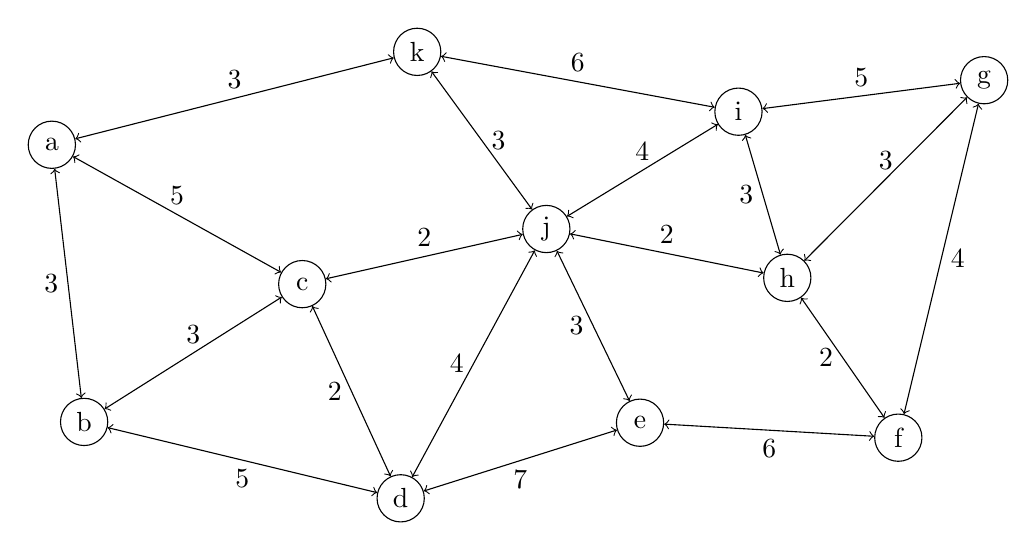
\begin{tikzpicture}
        % Nodes
        \node[circle, draw, minimum size=0.6cm, inner sep=0pt] at (1.60, -2.12)  (a)    {a};
        \node[circle, draw, minimum size=0.6cm, inner sep=0pt] at (2.01, -5.64)  (b)    {b};
        \node[circle, draw, minimum size=0.6cm, inner sep=0pt] at (4.78, -3.89)  (c)    {c};
        \node[circle, draw, minimum size=0.6cm, inner sep=0pt] at (6.03, -6.61)  (d)    {d};
        \node[circle, draw, minimum size=0.6cm, inner sep=0pt] at (9.07, -5.65)  (e)    {e};
        \node[circle, draw, minimum size=0.6cm, inner sep=0pt] at (12.35, -5.84)  (f)    {f};
        \node[circle, draw, minimum size=0.6cm, inner sep=0pt] at (13.44, -1.30)  (g)    {g};
        \node[circle, draw, minimum size=0.6cm, inner sep=0pt] at (10.94, -3.81)  (h)    {h};
        \node[circle, draw, minimum size=0.6cm, inner sep=0pt] at (10.32, -1.70)  (i)    {i};
        \node[circle, draw, minimum size=0.6cm, inner sep=0pt] at (7.88, -3.19)  (j)    {j};
        \node[circle, draw, minimum size=0.6cm, inner sep=0pt] at (6.24, -.94)  (k)    {k};


        \draw[<->]  (a) edge node[midway, left] {3} (b);
        \draw[<->]  (a) edge node[midway, above] {5} (c);
        \draw[<->]  (a) edge node[midway, above] {3}  (k);

        \draw[<->]  (b) edge node[midway, above] {3} (c);
        \draw[<->]  (b) edge node[midway, below] {5} (d);

        \draw[<->]  (c) edge node[midway, left] {2} (d);
        \draw[<->]  (c) edge node[midway, above] {2} (j);

        \draw[<->]  (d) edge node[midway, left] {4} (j);
        \draw[<->]  (d) edge node[midway, below] {7} (e);

        \draw[<->]  (e) edge node[midway, left] {3} (j);
        \draw[<->]  (e) edge node[midway, below] {6} (f);

        \draw[<->]  (f) edge node[midway, right] {4} (g);
        \draw[<->]  (f) edge node[midway, left] {2} (h);

        \draw[<->]  (g) edge node[midway, above] {3} (h);
        \draw[<->]  (g) edge node[midway, above] {5} (i);

        \draw[<->]  (h) edge node[midway, left] {3} (i);

        \draw[<->]  (i) edge node[midway, above] {4} (j);
        \draw[<->]  (i) edge node[midway, above] {6} (k);

        \draw[<->]  (j) edge node[midway, right] {3} (k);
        \draw[<->]  (j) edge node[midway, above] {2} (h);
    \end{tikzpicture}
    \caption{Beispielgraph}
\end{figure}

\todo{Graphen auf Kinderniveau erklären und schöne Bilder von Graphen zeigen}.

\section{Definitionen}
Damit in den nachfolgenden Kapiteln sinnvoll argumentiert werden kann, ist es notwendig, einige Begriffe zu definieren.

\begin{definition}[Graph]
    Sofern nicht anders angegeben, wird ein endlicher, gerichteter Graph mit Kantengewichten, ohne Mehrfachkanten und Schleifen, einfach als Graph bezeichnet.

    Als Schreibweise wird $G = (V, E)$ verwendet, wobei $V$ die Knotenmenge und $E$ die Kantenmenge ist. Eine Kante ist ein Tupel $(t, h, w)$. $t \in V$ wird als \emph{Fuß}, $h \in V$ als \emph{Kopf} und $w \in \mathbb{R}$ als \emph{Gewicht} bezeichnet. Gelegentlich wird auch nur $(t, h)$ geschrieben, um auszudrücken, dass zwei Knoten verbunden sind. Da ein Graph keine Mehrfachkanten zulässt, definiert diese Schreibweise auch eindeutig das Kantengewicht.

    Wird $G$ als ungerichtet bezeichnet, dann gilt $(t, h) \in E \Leftrightarrow (h, t) \in E$.
\end{definition}

In einem Graphen gibt es oft das Interesse, von einem Knoten zu einem anderen zu gelangen.
Diese Verbindungen zwischen Knoten werden durch sogenannte Wege dargestellt.

\begin{definition}[Weg]
    Ein Weg auf einem Graph $G = (V, E)$ ist eine Folge von Knoten $v_1, \dotsc, v_n$, für die gilt, dass benachbarte Knoten im Weg eine Kante in $E$ bilden.

    \todo{Wie nenne ich die Hoplänge?}

    Die Summe der Kantengewichte aller Kanten $(v_i, v_{i + 1})$ wird \emph{Länge} des Weges genannt. Der Knoten $v_1$ wird Startknoten, $v_n$ Zielknoten genannt.
\end{definition}

Zwischen zwei Knoten kann es mehrere unterschiedliche Wege geben.
Diese Wege können auch unterschiedliche Länge haben.

\begin{definition}[Kürzester Weg]
    Ein Weg $v_1, \dotsc, v_n$ ist \emph{ein kürzester Weg}, wenn die Länge des Weges unter allen Wegen von $v_1$ nach $v_n$ minimal ist. Die Länge des kürzesten Weges wird als \emph{Abstand} von $v_1$ und $v_n$ bezeichnet. Die Definition des Graphen lässt es zu, dass es mehrere kürzeste Wege zwischen zwei Knoten gibt.

    Sei $P \subset V \times V$ die Menge der Knoten, zwischen denen ein Weg existiert. Dann sind definiert:
    \begin{enumerate}
        \item
              ${spd} \colon P \to \mathbb{R}$ weist einem Knotenpaar den Abstand zu.

        \item
              ${sp} \colon P \to V \times V \times \dots \times V$ weist einem Knotenpaar einen kürzesten Weg zu.
    \end{enumerate}
\end{definition}

\begin{definition}[Umkehrgraph]
    Sei $G = (V, E)$ ein Graph. Dann ist $G^T = (V, E^T)$ mit $(t, h, w) \in E \Leftrightarrow (h, t, w) \in E^T$ der \emph{Umkehrgraph} von $G$.
\end{definition}

Zusätlich zum finden eines Weges zwischen zwei Knoten ist es häufig notwendig den kürzesten Weg von einem Knoten zu allen anderen Knoten zu finden.
Auch die Umkehrung dieses Problem ist interesannt, also die kürzesten Wege von allen Knoten zu einem zu bestimmen.
Diese Probleme sind äuivalent, da das Finden alle kürzesten Wege zu einem Knoten auf einem Graph $G$ dem Finden aller kürzester Wege auf dem Umkehrgraph $G^T$ entspricht.

\section{Nicht-Straßen Graphen}



Kürzeste Pfad Queries mit dem klassischen Dijksta Algorithmus sind auf den visibility Graphen deutlich teuerer als auf den triangulierten Graphen.


Fokus dieser Arbeit erklären.

Unterschiede zwischen Straßengraphen und NIcht-Straßengraphen erklären.
TODO Straßengrqaphen sind hierarchisch, aber was heist das genau.
TODO kann ich mit einer Metrik binär unterteilen ob ein GraPh hierarisch ist?

Die graph erklären, die ich mir speziell anschaue.
Trianguliereung erklären TODO Daniel?

Graphen zeichen, metriken zeichen.
Degree Plot
Hitting Set Plot?
Sonstige Metriken? TODO Funke


shasum graphen
6c00147bf26a2c37e50db857f4ce4ab565a236dd  aegaeis-ref-graph.fmi
acdf08813a59534840c605984e9c37875f77f32a  aegaeis-ref-visibility.fmi
b22697934378f6f8af7fb7bf3ae2812d7b0029ec  medi-ref-graph.fmi
77760c910a13f9dc056f4ef3f3f532b00286c52f  medi-ref-visibility.fmi
b9727caf46fd3407ce0b5e2b08b941dfb15f95f6  pata-ref-graph.fmi
89356e6e6411b8340375c3aa0fc949fb4e58ff44  pata-ref-visibility.fmi


\section{Dijkstra}

\todo{Dijkstra Algorithmus erklären und Dijkstra Paper zitieren}

Ziel ist nicht Dijktra selbst, sondern folgende Metriken erklären.

\todo{Dijkstra Rank}
\todo{Queue Pops}
\todo{Max Queue len}

\section{Datenstrukturen}

Verschieden Graph Strukturen

Grundlegende Idee:
Ein Interface Graph welches nur ausgehende Kanten kennt.
get edge distance, set edge distance

Dieses habe ich für verschiedene Graphen implementiert.
Wichtigste:
VecVec: Ein Vec. Jeder Vertex hat hat einen Eintrag vom Typ Vec in dem die kanten sortiert nach Head sind.
VecHashMap: Ein Vec. Jeder Vertex hat einen Eintrag vom Typ HashMap (Head, Distance).
Vec: Zwei Vec. Einer für (Head, Distance), zweiter für startindex, stopindex für Vec.
TODO Indexmap?

Häufig eine Abwägung wie schnell gequeriet werden kann vs wie schnell bearbeitet werden kann.


für reverse dijkstra uä muss aber auch Vorgänger bekannt sein.
Idee: Reversible Graph aus einem Vorwärtsgrapg und Rückwärtgraph
Beide sind aber grundätzlich gleiche Struktur. Daher ist Vorwärts und Rückwärtssuche gleiche Funktion.


Gleiches gilt für Contracted Graph. Zwei Graphen Upward Graph und Downward Graph. Downward Graph ist aber \"umgedreht\" zur Definition aus dem Paper, es wird also beides mal eine Vorwärtssuche gemacht.


\section{Archivierung}

Zum Speichern von Graphen wird ein Text Based Format benutzt.


Beliebig viele Kommentar lines
leere line
num Vertices
num Edges
Vertices
Edges

Suche
Für Dijkstra verscheidene Datenstrukturen getestet.
Data (predecessor, distance)
Queue (min heap)
is\_expanded

jeweils ein Interface.

TODO. Testen verschiedener Kombinationen.
TODO. Wann ist reuse of allocation sinvoll?
TODO Decrease key



\chapter{Contraction Hierarchies}\label{chapter:ch}

Eine Methode um in Graphen, inbesondere in Straßengraphen, sehr schnell kürzeste Pfade zu berechen, sind Contraction Hierachies.
Die von \cite{geisberger2008contraction} vorgestellte Methode nutzt ein änliches Konzept zu dem in \autoref{graphs:strassengraphen} vorgestellten Level auf.
Die Grundidee der Suche eines kürzesten Pfades ist ein Bidirectionale Suche, welche jeweils nur höhere Level besucht.
Durch diese Enschränkung des Suchhraums kann, je nach dem Graphentyp, ein Speedup mehrerer größenordnungen erreicht werden.

Wie zu sehen sein wird, lassen sich die klassischen Methoden zur Erstellung der benötigten DAtenstrukturen nur bedingt auf Sichtbarkeitsgraphen anwenden.
Daher wird im follgenden zuerst unabhängig der Erstellung argumentiert.

Contraction Hierarchies bauen auf der Notation eines \emph{Levels} auf.
Jedem Knoten wird ein Level zugeorndet.
Diese kann als ein Grad der Wichtigkeit verstanden werden:
Je höher ein Level ist, desto wichtiger ist der Knoten im Allgemeinen für das finden von kürzesten Pfaden.

\begin{definition}[Level]
    Sei $G = V, E$ ein Graph.
    Sei $L \subseteq \mathbb{N}$ mit $\abs{L} = \abs{V}$.
    Dann wird eine bijketive Funktion ${vtl} \coloneq V \to L$ \emph{vertex-to-level} Funktion genannt.
    Ihre Umkehrfunktion ${ltv}$ wird \emph{level-to-vertex} Funktion genannt.
\end{definition}

Die ein Level aus genau einem Knoten besteht, ist keine zwingen Notwendigkeit
So setzt \cite{vetter2009parallel} etwa mehrere Knoten auf einem Level, um das Preprocessing zu beschleunigen.
Die in dieser Arbeit verwende Einschränkung vereinfacht allerdings die argumentation.

Bassierend auf dem Level kann der \emph{upward Graph} definiert werden.
Der Name des upward Graphen ergibt sich daher, dass die Suche in einem upward Graph auf das Level bezogen nur \emph{aufwärts} geht.
Formal ist dieser definiert als:

\begin{definition}[Upward Graph]
    Sei $G = (V, E)$ und ${vtl}$ eine \emph{vertex-to-level} Funktion dazu. Dann ist $G_u = (V, E_u)$ ein \emph{upward Graph} zu $G$ wenn gilt:
    \begin{enumerate}
        \item\label{ch:definition:legal_edges}
        $E_u$ enthält nur Kanten $(t, h, w)$ mit $t, h \in V$ und $w \in \mathbb{N}$ für die ${vtl}(t) < {vtl}(h)$ und $w >= {spd}_{G}((t, h))$ gilt.
        Ist $\abs{{sp}((t, h))} > 2$, so nennen wir die Kante auch eine Abkürzung (\emph{Shortcut}).

        \item\label{ch:definition:upward}
        $E_u$ enthält mindestens alle Kanten $(t, h, {spd}_{G}((t, h)))$ mit $t, h \in V$, für die gilt, dass $h$ das größte und $t$ das zweitgrößte Level auf allen kürzesten Wege auf $G$ von $t$ nach $h$ hat.
    \end{enumerate}
\end{definition}


Betrachten wir das ganze an dem bereits definierten Beispielgraph.
Sei ${vtl}$ definiert durch die Abbildung \autoref{ch::fig::vtl_abbildung} definiert.
Durch Anwendung der Regel \ref{ch:definition:upward} ergibt sich der in \autoref{ch::fig::upward_graph} gezeigte upward Graph.
Es ist hierbei zu erwähnen, dass keine zusätzlichen Kanten nach \autoref{ch:definition:legal_edges} eingefügt wurden.

Der enstande Graph ist azyklisch, der nur Kanten enthält, deren Kopf ein größeres Level als ihr Fuß hat.
Die Anzahl der in einer Breitensuche gefunden Knoten ist geringer, als im Ursprungsgraph.
Diese beiden Eingeschaften sorgen dafür, dass eine Suche in einem upward Graph kostengünstiger sei kann.
Die in einem upward Graph gefunden kürzesten Pfade bilden eine untere Grenze für kürzeste Pfade.
Wie später \todo{hier} zu sehen sein wird, kann es auch teruere sein.

\begin{table}[ht]
    \centering
    \begin{tabular}{lllllllllllll}
        Vertex & a & b & c & d & e & f & g & h & i & j  & k & \\
        Level  & 8 & 7 & 3 & 6 & 2 & 5 & 1 & 4 & 0 & 10 & 9 &
    \end{tabular}
    \caption{${vtl}$ Beispielfunktion}
    \label{ch::fig::vtl_abbildung}
\end{table}


\begin{figure}[ht]
    \centering
    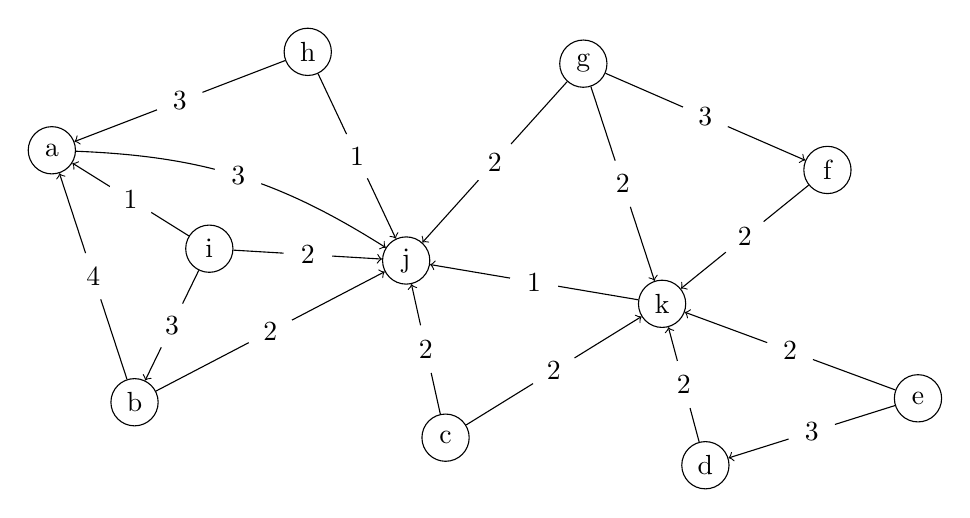
\begin{tikzpicture}
        % Nodes
        \node[circle, draw, minimum size=0.6cm, inner sep=0pt] at (0.5* 0.0, 0.5* 8.5)  (a)    {a};
        \node[circle, draw, minimum size=0.6cm, inner sep=0pt] at (0.5* 2.1, 0.5* 2.1)  (b)    {b};
        \node[circle, draw, minimum size=0.6cm, inner sep=0pt] at (0.5* 10.0, 0.5* 1.2)  (c)    {c};
        \node[circle, draw, minimum size=0.6cm, inner sep=0pt] at (0.5* 16.6, 0.5* 0.5)  (d)    {d};
        \node[circle, draw, minimum size=0.6cm, inner sep=0pt] at (0.5* 22.0, 0.5* 2.2)  (e)    {e};
        \node[circle, draw, minimum size=0.6cm, inner sep=0pt] at (0.5* 19.7, 0.5* 8.0)  (f)    {f};
        \node[circle, draw, minimum size=0.6cm, inner sep=0pt] at (0.5* 13.5, 0.5* 10.7)  (g)    {g};
        \node[circle, draw, minimum size=0.6cm, inner sep=0pt] at (0.5* 6.5, 0.5* 11.0)  (h)    {h};
        \node[circle, draw, minimum size=0.6cm, inner sep=0pt] at (0.5* 4.0, 0.5* 6.0)  (i)    {i};
        \node[circle, draw, minimum size=0.6cm, inner sep=0pt] at (0.5* 9.0, 0.5* 5.7)  (j)    {j};
        \node[circle, draw, minimum size=0.6cm, inner sep=0pt] at (0.5* 15.5, 0.5* 4.6)  (k)    {k};


        \draw[->]  (a) edge[bend left=15] node[circle, fill=white] {3} (j);

        \draw[->]  (b) edge node[circle, fill=white] {4} (a);
        \draw[->]  (b) edge node[circle, fill=white] {2} (j);

        \draw[->]  (c) edge node[circle, fill=white] {2} (j);
        \draw[->]  (c) edge node[circle, fill=white] {2} (k);

        \draw[->]  (d) edge node[circle, fill=white] {2} (k);

        \draw[->]  (e) edge node[circle, fill=white] {3} (d);
        \draw[->]  (e) edge node[circle, fill=white] {2} (k);

        \draw[->]  (f) edge node[circle, fill=white] {2} (k);

        \draw[->]  (g) edge node[circle, fill=white] {3} (f);
        \draw[->]  (g) edge node[circle, fill=white] {2} (j);
        \draw[->]  (g) edge node[circle, fill=white] {2} (k);

        \draw[->]  (h) edge node[circle, fill=white] {3} (a);
        \draw[->]  (h) edge node[circle, fill=white] {1} (j);

        \draw[->]  (i) edge node[circle, fill=white] {1} (a);
        \draw[->]  (i) edge node[circle, fill=white] {3} (b);
        \draw[->]  (i) edge node[circle, fill=white] {2} (j);


        \draw[->]  (k) edge node[circle, fill=white] {1} (j);
    \end{tikzpicture}
    \caption{Upward Graph des Beispielgraphs}
    \label{ch::fig::upward_graph}
\end{figure}

Die kürzeste Pfad Suche ist eine bidirectionale Suche, wobei die Suchen auf verschiedenen Graphen arbeiten.
Daher ist muss noch das Gegenstück das upward Graphens definiert werden, der \emph{downard Graph}.

\begin{definition}[Downward Graph]
    Sei $G = (V, E)$ und ${vtl} \coloneq V \to \mathbb{N}$ eine \emph{vertex-to-level} Funktion. Dann ist ein upward Graph des Umkehrgraphens $G^T$ ein \emph{downward Graph} zu $G$.
\end{definition}

Wenn ein Graph ungerichtet ist, dann er äuivalent zu seinem Umkehrgraphen.
Daher ist in so einem Fall dann auch der upward und downard Graph äuivalent.
Daher entspricht \autoref{ch::fig::upward_graph} gleichzeitig auch dem downward Graph des Beispielgraphens.

\section{Query}

Ein \emph{Contracted Graph} $C = (G_u, G_d)$ ist die Datenstruktur, mit deren Hilfe schnell kürzeste Wege gefunden werden können.
Sie besteht aus einem upwarward und downward Graph, wobei beide es eine ${vtl}$ Funktion geben muss, nach der Beide gültig sind.

Die Suche eines kürzesten Pfades von $a$ nach $e$ auf dem Beispielgraph gestaltet sich nun wie folgt:
Auf $G_u$ wird eine Breitensuche von $a$ und auf $G_d$ eine Breitensuche von $e$ durchgeführt.
Aus den von beiden besuchten Knoten wird derjenige ausgewählt, der die nidrigste Summe beider Distanzen hat.
Dieser Knoten auch auch das höchste Level auf dem Pfad.
\autoref{fig:ch:beispiel_suche} zeigt das auf- und absteigen der Level auf dem kürzesten Pfad.

\begin{figure}[ht]
    \centering
    \begin{tikzpicture}
        \node[circle, draw] at (0 * 1.5, -2 * 0.75)  (a)    {a};
        \node[circle, draw] at (1 * 1.5, -4 * 0.75)  (i)    {i};
        \node[circle, draw] at (2 * 1.5, -0 * 0.75)  (j)    {j};
        \node[circle, draw] at (3 * 1.5, -1 * 0.75)  (k)    {k};
        \node[circle, draw] at (4 * 1.5, -3 * 0.75)  (e)    {e};

        % draw axis
        \draw[->] (-1, -7 * 0.75) -- (-1, 0) node[above] {Level};

        \draw[->]  (a) -- (j);
        \draw[->]  (e) -- (k);
        \draw[->]  (k) -- (j);

        \draw[->, dotted]  (a) -- (i);
        \draw[->, dotted]  (i) -- (j);

    \end{tikzpicture}
    \caption{Beispiel einer Suche im Contrated Graph}
    \label{fig:ch:beispiel_suche}
\end{figure}

Diese informalle Beschreibung lässt sich formal definieren:

\begin{algorithm}
    \caption{Construction Hierachies Query}
    \begin{algorithmic}[1]
        \Require Upward-Graph $G_u = (V, E_u)$, Downward-Graph $G_d = (V, E_d)$, Startknoten $s \in V$, Zielknoten $t \in V$
        \Ensure Treffknoten $m \in V \cup \{ {none} \}$, ${dist}_u$, ${pre}_u$, ${dist}_d$, ${pre}_d$
        \State ${dist}_u$, ${pre}_u$ $\leftarrow$ Dijkstra$(G_u, s)$
        \State ${dist}_d$, ${pre}_d$ $\leftarrow$ Dijkstra$(G_d, t)$

        \State
        \State $m \leftarrow {none}$
        \State $d \leftarrow \infty$
        \State

        \ForAll {$v \in V$}
        \If {${dist}_u(v) + {dist}_d(v) < d$}
        \State $m \leftarrow v$
        \State $d \leftarrow {dist}_u(v) + {dist}_d(v)$
        \EndIf
        \EndFor

        \State
        \State \Return $m$, ${dist}_u$, ${pre}_u$, ${dist}_d$, ${pre}_d$
    \end{algorithmic}
    \label{ch:query_simple}
\end{algorithm}

Doch warum ist dies Korrekt?

\begin{beweis}
    Der Beweis der Korrektheit folgt in zwei Schritte.

    \begin{enumerate}
        \item
              Es existiert ein kürzester Pfad von $u$ nach $v$ in $G$ $\Rightarrow$ Er wird in $C$ gefunden.

              Da ${vtl}$ injektiv ist, existiert genau ein Knoten $t$ mit dem höchstem Level. Zerscheide den Pfad $(u, \dotsc, v)$ in zwei Teile:  und $(u, \dotsc, t)$ und $(t, \dotsc, v)$.

              Die Tupel benachbarten Knoten in $(u, \dotsc, t)$ sind nach der Definition des upward Graph Kanten von $G_u$. Daher wird $t$ im upward Graph gefunden.

              Analog dazu wird $t$ in $G_d$ gefunden, die Tupel benachbarter Knoten im Pfad $(v, \dotsc, t)$ sind nach der Definition des downward Graphs Kanten von $G_d$.

              Da die Tupel Kanten der Graphen sind, finden die Breitensuchen den Knoten $t$ mit minimalen Kosten ausgehend von $u$ bzw. $v$. Da $t$ auf dem kürzesten Pfad liegt, ist damit auch der kúrzeste Pfad von $u$ nach $v$

        \item
              Es existiert kein kürzester Pfad von $u$ nach $v$ in $G$ $\Rightarrow$ Es wird in $C$ kein Pfad gefunden gefunden.

              Angenommen, es würde ein Pfad in C gefunden werden. Die Tupel benachbarter Knoten des Pfades müssten dann Kanten in C sein.
              Mindestens einer diese Kanten hätte dann ein Gewicht welches gegen \autoref{ch:definition:legal_edges} der Definition verstoßt.
    \end{enumerate}

    Daher gilt, die Suche der kürzesten Pfad Distanz in $C$ ist äquivalent zu der in $G$
\end{beweis}

\subsection{Pfad gewinnung}
Bisher enthält der Pfad Shortcuts.
Entweder man ersetzt dan Shortcut auf einmal durch alle Knoten, oder iterativ durch jeweils zwei Kanten.

Diese müssen ersetzt werden.
Das geht, indem einen Stapel hat und shortcuts einfügt.

\section{Early stop}

Dass beide Suchen vollständig asugeführt werden ist nicht optimal.
Besser wäre es, frühzeitig stoppen zu können.
Vielleicht, wenn ein Knoten $t$ mit Distanz $d$ gefunden wurde.
Dann stoppen wenn top queue forward + top queue reverse >= d?
Das funktioniert nicht.
Denn bei der während bei einer normalen bidirectionale Suche sich die Fronten treffen, kann eine CH suche auch hinter die Front der anderen gelangen.

Daher ist die Abbruchbedingung: top queue >= d.

Todo: Abbruch mit Heuristik. Wenn ich upper bound kenne. breche ab top queue >= upper bound.

\todo{Funke fragen}.

\section{Pruning}


% https://cstheory.stackexchange.com/questions/23767/why-is-label-pruning-possible-with-hub-labeling
Aus dieser Definition folgt, dass der kürzeste Pfad zwischen zwei Knoten in $G_u$ ist also mindestens genausolang ist wie in $G$.
Der Pfad darf aber auch länger sein.

\todo{Zeiche zwei Suchbäume, jeweils in G und Gu}

Für die Suche sind aber nur Knoten interesannt, die tatsächlich kürzesten Pfad Abstand haben.

Wie kann man diese Knoten nun leicht rausfiltern?
Beim expanded eines Knoten prüft man, für die Nachbarn der Gegenrichtung:
\todo{Funke nochmal die Details}


\section{Erstellung}

Das Ziel der Contraction Hierarchies ist es aus dem Graph zwei Teilgraphe mit Abkürzungen (\emph{shortcuts}) zu erstellen.
Auf diesen Graphen kann mit einer Breitensuche effizient ein Knoten gefunden werden, der auf dem kürzesten Pfad zwischen zwei Knoten liegt.

\subsection{Contraction}

Der Name Contraction Hierachies leitet sich aus Konzept der Knoten Kontraktion (contraction) ab.
Diese funktioniert wie folgt:

\begin{definition}[Vertex Contraction]
    Sei $G = (V, E)$ ein Graph. Sei $v \in V$ der zu kontraktierende Knoten. Er wird kontraktiert indem:

    \begin{enumerate}
        \item\label{ch:contraction:when_shortcut}
        für jeden Vorgänger $u \in V$ und jeden Nachfolger $w \in V$ von $v$ einen Kante $(v, w, {spd}(u, w))$ in $E$ eingefügt wird, wenn $v$ auf dem einzigen kürzesten Pfad zwischen $u$ und $v$ liegt. Diese Kanten sind Shortcuts.

        \item
              alle Kanen von und zu $v$ entfernt werden.
    \end{enumerate}

    $v$ ist danach isoliert.
\end{definition}

Diese Operation erhält für die verbleibenden Knoten die kürzesten Pfade.
Betrachten wir dies wieder am Beispielgraph.
Sei $i$ der zu kontraktierende Knoten, die Nachbarn sind $a$, $b$, $j$ und $h$.
Die kürzesten Pfade von $(a, b)$, $(b, j)$, $(h, j)$ und $(a, h)$ fürhren nicht durch $i$.
Der von $(a, j)$ jedoch doch, daher wird eine Kante eingefügt.
\autoref{graphs:fig:example_contraction} zeigt den Graphen nach der Kontraktion.

\begin{figure}[ht]
    \centering
    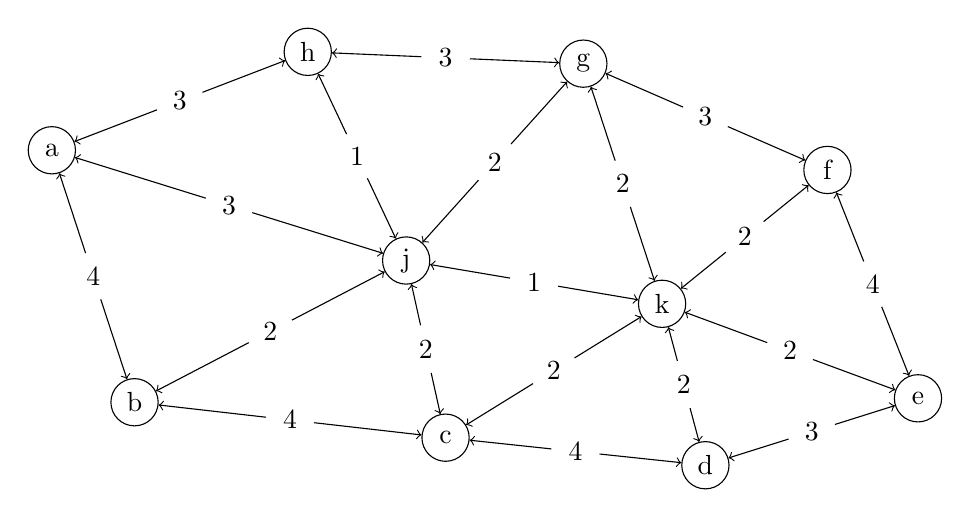
\begin{tikzpicture}
        % Nodes
        \node[circle, draw, minimum size=0.6cm, inner sep=0pt] at (0.5* 0.0, 0.5* 8.5)  (a)    {a};
        \node[circle, draw, minimum size=0.6cm, inner sep=0pt] at (0.5* 2.1, 0.5* 2.1)  (b)    {b};
        \node[circle, draw, minimum size=0.6cm, inner sep=0pt] at (0.5* 10.0, 0.5* 1.2)  (c)    {c};
        \node[circle, draw, minimum size=0.6cm, inner sep=0pt] at (0.5* 16.6, 0.5* 0.5)  (d)    {d};
        \node[circle, draw, minimum size=0.6cm, inner sep=0pt] at (0.5* 22.0, 0.5* 2.2)  (e)    {e};
        \node[circle, draw, minimum size=0.6cm, inner sep=0pt] at (0.5* 19.7, 0.5* 8.0)  (f)    {f};
        \node[circle, draw, minimum size=0.6cm, inner sep=0pt] at (0.5* 13.5, 0.5* 10.7)  (g)    {g};
        \node[circle, draw, minimum size=0.6cm, inner sep=0pt] at (0.5* 6.5, 0.5* 11.0)  (h)    {h};
        % \node[circle, draw, minimum size=0.6cm, inner sep=0pt] at (0.5* 4.0, 0.5* 6.0)  (i)    {i};
        \node[circle, draw, minimum size=0.6cm, inner sep=0pt] at (0.5* 9.0, 0.5* 5.7)  (j)    {j};
        \node[circle, draw, minimum size=0.6cm, inner sep=0pt] at (0.5* 15.5, 0.5* 4.6)  (k)    {k};


        \draw[<->]  (a) edge node[circle, fill=white] {4} (b);
        \draw[<->]  (a) edge node[circle, fill=white] {3} (h);
        \draw[<->]  (a) edge node[circle, fill=white] {3} (j);

        \draw[<->]  (b) edge node[circle, fill=white] {4} (c);
        \draw[<->]  (b) edge node[circle, fill=white] {2} (j);

        \draw[<->]  (c) edge node[circle, fill=white] {4} (d);
        \draw[<->]  (c) edge node[circle, fill=white] {2} (j);
        \draw[<->]  (c) edge node[circle, fill=white] {2} (k);

        \draw[<->]  (d) edge node[circle, fill=white] {3} (e);
        \draw[<->]  (d) edge node[circle, fill=white] {2} (k);

        \draw[<->]  (e) edge node[circle, fill=white] {4} (f);
        \draw[<->]  (e) edge node[circle, fill=white] {2} (k);

        \draw[<->]  (f) edge node[circle, fill=white] {3} (g);
        \draw[<->]  (f) edge node[circle, fill=white] {2} (k);

        \draw[<->]  (g) edge node[circle, fill=white] {3} (h);
        \draw[<->]  (g) edge node[circle, fill=white] {2} (j);
        \draw[<->]  (g) edge node[circle, fill=white] {2} (k);

        \draw[<->]  (h) edge node[circle, fill=white] {1} (j);

        \draw[<->]  (j) edge node[circle, fill=white] {1} (k);
    \end{tikzpicture}
    \caption{Beispielgraph}
    \label{graphs:fig:example_contraction}
\end{figure}

Um einen Contracted Graph zu erstellen, werden alle Knoten kontraktiert, wobei die Kanten, die in jedem Schritt entfernt werden, gesammelt werden.
Die Kanten, deren Kopf-Level größer ist, bilden die Kanten des upward Graphens.
Die übrigen Kanten, also die deren Fußlevel größer ist, werden invertiert und bilden die Kanten des downard Graphens.

Diese Art der Erstellung erzugt zulässige upward Graphen, da die eingefügten Shortcuts die die Bedingung aus \autoref{ch:definition:upward} erfüllen.
Es ist jedoch möglich, dass Kanten eingefügt werden, die nicht notwendig sind.
Insbesondere hat die Reihenfolge der Kontraktion einen großen Einfluss auf die Qualität der erzeugten Graphen.
\todo{Wie definiere ich die Qualität}?

Die Suche in der Kontraktion wird häufig wie folgt gestalltet.
Es wird eine one-to-many Suche gemacht, welche auf zwei Arten limitiert ist:
Es wird nur der Ball mit Abstand der gößten Distanz out-Kanten + in-Kante abgesucht.
Die Anzahl der Hops wird begrenzt.
Dadurch werden im Zweifelsfall mehr Kanten als benötigt eingefügt, dies ist aber schneller.

\subsubsection{Top-Down}

Bei der Top-Down Contraction ist level-to-vertex Funktion ${ltv}$ vorgegeben.
Die Knoten werden in Reihenfolge ihres Levels kontrakiert, wobei mit dem niedrigsten Level begonnen wird.

\paragraph{Zufällig sortiert}
Die Knoten werden zufällig auf die Level verteilt

\paragraph{Sortiert nach Grad}
Die Knoten werden nach ihrem Grad sortiert, wobei die kleinsten Grade zuerst kontraktiert werden.
Die überlegung dahinter ist, dass Knoten mit vielen Nachbarn auch viele neue Kanten einfügen können, was vermieden werden soll.

\paragraph{Hitting Set}
Es wird ein Hitting Set über Pfade in $G$ erstellt.
Die Knoten welche am wenigsten Pfade treffen, werden zuerst kontraktiert.
Dies ist potentiell eine der besten Lösungen \todo{Oder? Kann man das beweisen?}.

\subsubsection{Bottom-Up}

Bei der Bottom-Up contraction wird die vertex-to-level Funktion ${vtl}$ währen der Kontraktion erstellt.
Dafür wird mit einer Heuristik der jeweils nächst \emph{unwichtigste} Knoten ausgewählt, kontraktiert und dem nächstem Level zugewiesen.
Ein unwichtiger Knoten hat hierbei einen niedrigen Heuristik-Wert.
Hier hängt die Qualität der des Ergebnis von der Heuristik ab.

Da das Neuberechnen des Heuristik für alle Knoten im Allgemeinen zu teuer ist, werden zwei Methoden angewendent:
Beim \emph{Lazy poping} besteht die Annahme, dass ein Knoten nur wichtiger werden kann.
Aus der Warteschlange wird ein Knoten entnommen und geprüft, ob sein Heuristik-Wert noch gleich ist.
Wenn er noch gleich ist, wird er kontraktiert, wenn nicht wird er zurück die Warteschlange gepusht.
Dies wird wiederholt, bis schließlich ein Knoten gefunden wird.
Beim \emph{Neighbor update} werden nach der Kontraktion eines Knoten die Heuristik Werte der Nachbarn geupdated.

Es sind viele Heurisiken Möglich, die auch kombiniert werden können.
Die in der Praxis am meist-verwendet Heurisik ist die \emph{Kanten-Differenz}.
Sie gibt an wie sich die Anzal der Kanten im gesammten GRaph verändert
Sie wird durch die Anzahl der hinzugefügten Kanten subtrahiert durch die Anzalh der entfernten Kanten gebildet.
Hierfür wird die Kontraktion eines Knoten simuliert.

\subsubsection{Ideen}

Die bisher erwähnten Methoden eignen sich nur bedingt für graphen mit großem durchscnittlichen Knotengrad.
Für die Kontraktion muss jeweils für jeden Vorgänger eine Suche zu jedem Nachfolger gemacht werden.
Insbesonder für Sichtbarkeitsgraphen ist das sehr teuer.

Es gibt zwei Stellen, die beschleunigt werden müssen:
Ordering Heuristik und Kontraktion

\paragraph{Kontraktion}
Anstatt einer Suche, verwende eine Upper Bound Heuristic.
Es muss ein Shortcut eingefügt werden, wenn die Shortcut Distanz gleich der Wahren Distanz ist.
Dies ist erfüllt, wenn die Shortcut Distanz kleiner gleich einer Upper Bound ist.
Zusätzlich gilt, wenn lower bound == shortcut distanz, dann muss Shortcut eingefügt werden.

Dafür gibt es zwei Ideen, die kombiniert werden können.
Landmarks und eine CH/HL des triangulierten Graphes für den Sichtbarkeitsgraph.
Vielleicht gilt, dass Landmarks für größere Entfernungen / mehr Hops gut ist und CH/HL für kleine?

Alternativ, aber wahrscheinlich super doof:
Füge jeden Shortcut ein.

Heuristic.
Statt suche kann man auch heursitc benutzten.

Used heuristics:
TrivialeHeuristic (all in). Füge jeden shortcut ein.

\paragraph{Ordering Heuristik}
Wähle $n$ Paara aus Vorgänger Nachgänger aus und erstelle für diese Edge Differnce (wieder mit Heuristik).
\todo{plot genauigkeit vs Zeit, vielleicht über so 1000 Knoten?}

\section{Brute force}

Die upward Graphen können auch stumpf berechnet werden.
Dafür wird pro Knoten eine (zwei, upward, downard) Dijsktrasuche gemacht, bis alle Knoten nach der Bedingung gefunden werden.


Dafür wird während der Dijstra Suche notiert, was das größte Level auf dem Weg von der Wurzel bis zu dem Knoten ist.
Ein Knoten ist der Kopf eine CH Kante, für die gilt, dass das größte Level auf dem Weg zur Wurzel zu ihr sie selber hat und der größte Level des Vorgängers der der Wurzel ist.
Das Gewicht der Kante kann Dijkstra entommen werden.
Wenn für Knoten ein max Level auf dem Pfad haben, welches größer als das der Wurzel ist, kann abgebrochen werden.

Die Shortcuts können dabei auch erstellt werden.
Der zu shortcutende Knoten ist der, mit demm dritthöchstem Level dazwischen.
Die anderen müssen auch erstellt werden, denn sonst kannes Probleme geben: \todo{Bild}

Das mit den Shortcuts ist dann nicht so einfach. TODO Bild


\chapter{Kontraktion in Sichtbarkeitsgraphen}\label{chapter:kontraktion}

Die zuvor beschriebene Kontraktion von Knoten und Graphen ist bei Graphen mit hohen Knotengraden, wie zum Beispiel Sichtbarkeitsgraphen, deutlich rechenintensiver als bei Graphen mit geringeren Knotengraden, wie etwa Straßengraphen.
Für die Knoten-Kontraktion muss für jeden Vorgängerknoten eine Dijkstra-Suche durchgeführt werden, und für jedes Paar aus Vorgänger und Nachfolger ist zu prüfen, ob eine Abkürzung eingefügt werden muss.
Ein hoher Knotengrad bedeutet somit viele Dijkstra-Suchen und zahlreiche Vergleiche, ob eine Abkürzung notwendig ist.

Bei der Bottom-Up-Kontraktion wird die Kontraktion potenziell mehrfach simuliert, bevor sie wirklich ausgeführt wird.
Bei Lazy-Popping werden die Knoten oft nicht kontraktiert, sondern mit aktualisiertem Heuristik-Wert in die Warteschlange zurückgeschoben.
Beim Neighbor-Update sind jeweils sehr viele Nachbarn zu aktualisieren.
Auch das Einfügen und Löschen von Kanten stellt hierbei einen nicht zu vernachlässigenden Zeitfaktor dar.

Um Graphen mit hohen Knotengraden effizient zu kontrahieren, ist es entscheidend, die Kontraktion einzelner Knoten zu beschleunigen und eine effizient sowie effizient erstellbare Reihenfolge der Kontraktionen zu finden.
Auch die zur Repräsentation von Graphen verwendeten Datenstrukturen sollten betrachtet werden, damit das Finden von Nachbarn sowie das Einfügen und Löschen von Kanten effizient und parallel möglich ist.

\section{Kontraktion mit oberer Schranke}
Anstelle einer potenziell rechenintensiven Dijkstra-Suche pro Vorgänger kann eine Heuristik pro Paar aus Vorgänger und Nachfolger eine obere Schranke für den Abstand geben.
Eine Kante als Abkürzung wird dann eingefügt, wenn ihre Länge kleiner oder gleich der berechneten oberen Schranke für den Abstand ist.
Damit dies für die Kontraktion eines einzelnen Knotens effizienter ist, muss die Ermittlung der Heuristik für alle Paare eines bestimmten Vorgängers und aller Nachfolger schneller sein als die Dijkstra-Suche.
Damit die Kontraktion des gesamten Graphen effizient bleibt, müssen die Folgekosten unnötiger Kanten geringer sein als der Zeitgewinn durch den Einsatz der Heuristik.
Im Folgenden werden verschiedene Heuristiken diskutiert.

\subsection{Triviale Heuristik}
Die \emph{Triviale Heuristik} setzt die obere Schranke für jedes Knotenpaar auf $\infty$.
Dies bedeutet, dass für jedes Paar aus Vorgänger und Nachfolger, unabhängig von der tatsächlichen Distanz, eine Kante als Abkürzung eingefügt wird.
Unter der Annahme, dass in Graphen mit sehr hohem Knotengrad fast alle Nachbarn bereits mit einer Kante verbunden sind, könnte der Anteil der unnötig eingefügten Abkürzungen im Vergleich zu den notwendigen vernachlässigbar sein.

\subsection{Vereinfacher Graph}
Sei $G = (V, E)$ der zu kontrahierende Graph.
Lässt sich zu $G$ effizient ein vereinfachter Graph $G' = (V, E')$ mit $\forall s, t \in V \colon {spd}_{G'} ((s, t)) \geq {spd}_{G} ((s, t))$ konstruieren, so kann dieser zur Berechnung der oberen Schranke verwendet werden, etwa indem die Dijkstra Suchen auf ihm ausgeführt werden.
Alternativ kann $G'$ auch in einen Contracted- oder Hub-Graph umgewandelt werden, womit die obere Schranke dann für jedes Vorgänger Nachfolger Paar einzelnen berechnet wird.

Für Graphen in der euklidischen Ebene sind Triangulierungen aber leicht zu erstellen.
\todo{Weiter}

Weitere Methoden zur Vereinfachung eines Graphen, ohne den Abstand zwischen zwei Knoten zu verkleinern, werden in dieser Arbeit nicht weiter behandelt.
Es ist anzunehmen, dass die Genauigkeit der oberen Schranke und die Geschwindigkeit der Berechnungen auf dem vereinfachten Graphen im Widerspruch stehen.
Weiter sind solche vereinfachten Graphen im Allgemeinen schwer zu konstruieren.

Diese Methode lässtich besonders gut auf die in dieser Arbeit bearbeiteten Sichtbarkeitsgraphen und ihre Triangulierungen anwenden, da Triangulierungen eine obere Schranke für Sichtbarkeitsgraphen liefern und Berechnungen auf ihnen im Vergleich sehr effizient sind.

\subsection{Dreiecksungleichung}
Ähnlich zu ALT\cite{goldberg2005computing} kann eine Menge \emph{Hubs} berechnet werden, welche mittels der Dreiecksungleichung eine obere Schranke angeben können.
Ein Hub ist hierbei ein Knoten $l \in V$, für den die Distanz zu und von allen Knoten bekannt ist, die obere Schranke des Abstandes zweier Knoten $s, t \in V$ kann dann durch ${spd}_G ((u, l)) + {spd}_G ((l, u))$ berechnet werden.
Liegt $l$ dabei auf einem kürzesten Pfad von $u$ nach $v$, so entspricht der Wert sogar genau dem der kürzesten Pfad Distanz.
Die obere Schranke über mehrere Hubs wird durch die Wahl der kleinsten oberen Schranken bestimmt.
In der Implementation hierfür reicht es sogar, eine obere Schranke zu finden, die kleiner als die potenzielle Abkürzung ist, diese kann dann keine optimale Abkürzung sein.

Die Hubs können dabei über die Berechnung eines Hitting-Sets bestimmt werden.
Durch die Auswahl von Hubs auf diese Art steigt die Genauigkeit der oberen Schranken mit der Hop-Länge der kürzesten Pfade, da die Wahrscheinlichkeit, dass diese durch einen Hub getroffen wird, steigt.
Durch mehr Hubs steigt allerdings auch der Zeitbedarf der Berechnung der oberen Schranke.

\subsection{Kombination mehrer oberer Schranken}
Sind für eine Graph mehrere Heuristiken bekannt, so so kann für eine potenzielle Abkürzungen aus allen oberen Schranken die kleinste ausgewählt werden.
Dies ist besonders dann sinvoll, wenn die Heuristiken jeweils eine Teilmenge alle Knotenpaare gut abdecken.
Insbesondere die Kombination von Dreicksungleichung und vereinfachtem Graph ist hierbei erfeolgsversprechen unter der Annahme, dass die erste für große und zweitere für kleine Hop-Abstände gute obere Schranken liefert.

\section{Bottom-Up Heuristik}

Damit die Nachfolgenden Kontraktion einfacher werden ist nicht die Kanten Differenz interesannt, sondern $\sum_{n \in \text{Nachbarschaft}(v)} (\text{Grad}_\text{neu}(n))^2 - (\text{Grad}_\text{alt}(n))^2$.
Der Kantendifferenz ist es egal, dass alle neue Kanten zu einem einzigen Knoten gehen. Dieser Heuristik nicht.

% TODO das drinnne lassen?
% \section{Datenstrukturen}
% 
% Im Allgemeinen haben wir zwei Anforderungen an die verwendeten Datenstrukturen, welche zur Repräsentation der Graphen verwendet werden: Es muss möglich sein für einen Knoten seine Vorgänger und Nachfolger zu finden und es muss möglich sein Kanten zu verändern oder zu entfernen.
% Diese beiden Ansprüche stehen sich mitunter gegenüber.
% 
% Knoten und Distanzen werde in der Implentierung als uint32 repräsentiert.
% Als Grundbaustein wurden verschiedene Graphen implementiert, welche jeweils nur ihre Nachfolger kennen.
% Damit ein Graph auch seine Vorgänger kennt, wurden jeweils zwei dieser Graphen zusammen benutzt.
% 
% \subsection{VecVecGraph}
% 
% Ein VecVecGraph besteht aus einem Vektor mit jeweils einem Eintrag pro Knoten.
% Dieser Eintrag ist ein Vector über Tuple Knoten $\times$ Distanz, welche nach dem Knoten sortiert sind.
% Der Knoten entspricht dabei dem Kopf einer Kante, ihr Fuß ist der Index in dem ersten Vektor.
% Soll eine Kante gefunden werden, so muss im Vektor, welche mit dem Fuß gefunden wird, eine Binäre Suche nach dem Kopf gemacht werden.
% 
% Das Iterieren über von aus einem Knoten ausgehenden Kanten ist damit effizient, das finden einer bestimmten Kante für kleinere Grade auch.
% Bei größeren Graden kann die Binäre Suche jedoch eine einen negativen Perfomance Overhead darstellen.
% Gleiches gilt für das Einfügen von neuen und Löschen von bestehenden Kanten, denn für größere Grade müssen dafür eine größere Menge an Knoten geschoben werden.
% 
% \subsection{VecHashGraph}
% 
% Ein VecHashGraph besteht wieder aus einem Vektor mit jeweil einem Eintrag pro Knoten, welcher eine HashMap Knoten auf Distanz ist.
% Durch die ausgehenden Kanten kann dann iteriert werden, indem die HashMap, welche zum Fuß gehört aufgerufen wird und durch diese itertiert wird.
% 
% Das Iterieren über diese Kanten ist etwas ineffizienter, da die Einträge in der HashMap nicht konitunierlich im Speicher liegen und dadurch die Cache-Effizent sinkt.
% Dafür wird bei größeren Graden das Finden von spezifischen Kanten, sowie das Einfügen und Löschen effizenter.
% Eine in dieser Arbeit nicht benutzte aber interesannte Datenstruktu ist die HashMap, Effizientes Iterieren und Finden von Kanten mit inefieziennten Einfügen und Löschen verbindet.
% 
% \subsection{VecGraph}
% 
% Soll ein Graph nicht verändert werden, sondern nur zum Finden von Nachbarn in einer Dijkstra Suche benutxt werden, so bietet sich ein VecGraph an.
% Dieser besteht aus zwei Vectoren, einem Index Vektor mit je einem Eintrag pro Knoten der Form Startindex, Stopindex und einem Kanten Vector der Form Knoten, Distanz.
% Aus einem Knoten ausgehende Kanten lassen sich dann finden, indem im Indexvektor der Start- und Stopindex gefunden wird.
% Dieses Paar gibt an, wo im Kantenindex die dazugehörigen Kanten sind.
% Durch die Verwendung des Start- undt Stopindex lassen sich die Kanten von häufig benutzten Knoten an einem Ende des Knotenvektors grupieren, dadurch lässt sich die Wahrscheinlichkeit von Cache-Hits erhöhen.
\chapter{PEOPLE: Predetermined Order, Prunded Label}\label{chapter:peopel}

Wie im \autoref{chapter:kontraktion} diskutiert wurde, ist Kontraktion von Graphen mit hohem durschnitlichen Knotengrad aufwendig.
Vielleicht ist die Kontraktion von ihnen sogar so aufwendig, dass sie sich nicht in sinvoller Zeit kontrahieren lassen
Trotzdem wäre es praktisch, wenn sich die Anfrage-Zeiten von Contraction Hierarchirs und Hierachical Hub Labeling auch auf sie übertragen ließen.
Hierfür charakterisieren wir den Contracted- und Hub-Graphen neu und stellen anschließend PEOPLE (\textbf{P}redetermined \textbf{O}rder, \textbf{P}runded \textbf{L}ab\textbf{e}l) vor, eine Methode wie Hub- und Contracted-Graphen mit einer vorgegeben vertex-to-level-Funktion ohne Knoten-Kontraktion erstellt werden können.

Um die Nachfolgende Definition vorzubereiten, betrachten wir ein Beispiel.
Sei $G = (V, E)$ mit $V \supset \{ u, v, w \}$ und $E = \{ (u, v, {spd}((u, v))), (v, w, {spd}((v, w))) \}$, ein Produkt einer Kontraktion, also zu Beginn mehr Kanten und nicht-isolierte Knoten entiehlt
Es soll nun $v$ kontraktiert werden.
Hierfür wir eine Kante $(u, w, {spd}((u, w)))$ eingefügt und die Kanten $(u, v), (v, w)$ entfernt.
Daraus können zwei Folgerungen gezogen werden:

\begin{enumerate}
  \item
    Es gibt einen kürzesten Pfad von $u$ nach $w$ in $G$ für den gilt, dass alle Knoten zwischen $u$ und $w$ bereits kontrahiert wurden.
    Diese haben daher auch ein niedrigeres Level als $u$ und $u$.

  \item
    $(u, w) \in E_u$ gilt genau dann, wenn $w$ das größte Level auf allen Pfaden von $u$ nach $w$.
    $(w, u) \in E_d$ gilt, wenn $u$ das größte Level hat.
\end{enumerate}

Basierend auf dieser Überlegung, definieren wir den Upward-Graph neu.

\begin{definition}[Upward-Graph]\label{people:def:upward_graph}
  Sei $G = (V, E)$ und ${vtl}$ eine vertex-to-level Funktion dazu.
  Dann ist $G_u = (V, E_u)$ ein \emph{Upward-Graph} zu $G$ wenn für jeden Knoten $t \in V$ gilt:

  \begin{itemize}
    \item
      $E_u$ enthält nur Kanten $(t, h, d)$ mit $h \in V$ und $d \in \mathbb{R}^+$, für die es einen $t$-$h$ Pfad der Länge $d \geq {spd}_G (t, g)$ gibt, so dass auf ihm $h$ das größte und $t$ das zweitgrößte Level hat.

    \item
      $E_u$ enthält alle Kante $(t, h, {spd}_G (t, h))$ mit $h \in V$, für die gilt, dass auf \emph{allen} $t$-$h$ Pfaden $h$ das größte und $t$ zweitgröste Level hat.
  \end{itemize}
\end{definition}

Betrachten wir dies wieder am Beispielgraph.
Sei ${vtl}$ definiert durch die Abbildung in \autoref{ch::fig::vtl_abbildung} definiert.
Durch Anwendung der neuen Definition des Upward-Graph ergibt sich der in \autoref{ch::fig::upward_graph} gezeigte Graph.

\begin{table}[ht]
  \centering
  \begin{tabular}{lllllllllllll}
    Vertex & a & b & c & d & e & f & g & h & i & j  & k & \\
    Level  & 8 & 7 & 3 & 6 & 2 & 5 & 1 & 4 & 0 & 10 & 9 &
  \end{tabular}
  \caption{${vtl}$ Beispielfunktion}
  \label{ch::fig::vtl_abbildung}
\end{table}

\begin{figure}[ht]
  \centering
  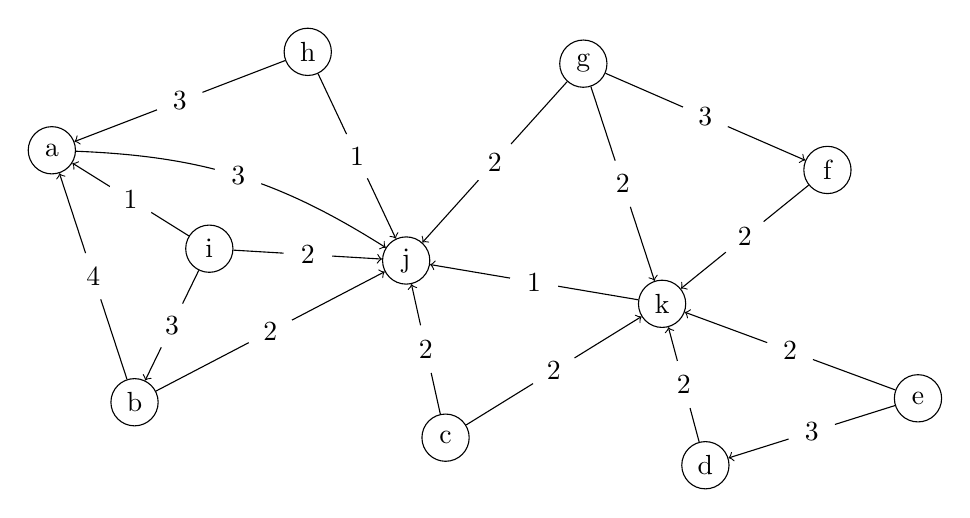
\begin{tikzpicture}
    % Nodes
    \node[circle, draw, minimum size=0.6cm, inner sep=0pt] at (0.5* 0.0, 0.5* 8.5)  (a)    {a};
    \node[circle, draw, minimum size=0.6cm, inner sep=0pt] at (0.5* 2.1, 0.5* 2.1)  (b)    {b};
    \node[circle, draw, minimum size=0.6cm, inner sep=0pt] at (0.5* 10.0, 0.5* 1.2)  (c)    {c};
    \node[circle, draw, minimum size=0.6cm, inner sep=0pt] at (0.5* 16.6, 0.5* 0.5)  (d)    {d};
    \node[circle, draw, minimum size=0.6cm, inner sep=0pt] at (0.5* 22.0, 0.5* 2.2)  (e)    {e};
    \node[circle, draw, minimum size=0.6cm, inner sep=0pt] at (0.5* 19.7, 0.5* 8.0)  (f)    {f};
    \node[circle, draw, minimum size=0.6cm, inner sep=0pt] at (0.5* 13.5, 0.5* 10.7)  (g)    {g};
    \node[circle, draw, minimum size=0.6cm, inner sep=0pt] at (0.5* 6.5, 0.5* 11.0)  (h)    {h};
    \node[circle, draw, minimum size=0.6cm, inner sep=0pt] at (0.5* 4.0, 0.5* 6.0)  (i)    {i};
    \node[circle, draw, minimum size=0.6cm, inner sep=0pt] at (0.5* 9.0, 0.5* 5.7)  (j)    {j};
    \node[circle, draw, minimum size=0.6cm, inner sep=0pt] at (0.5* 15.5, 0.5* 4.6)  (k)    {k};

    \draw[->]  (a) edge[bend left=15] node[circle, fill=white] {3} (j);

    \draw[->]  (b) edge node[circle, fill=white] {4} (a);
    \draw[->]  (b) edge node[circle, fill=white] {2} (j);

    \draw[->]  (c) edge node[circle, fill=white] {2} (j);
    \draw[->]  (c) edge node[circle, fill=white] {2} (k);

    \draw[->]  (d) edge node[circle, fill=white] {2} (k);

    \draw[->]  (e) edge node[circle, fill=white] {3} (d);
    \draw[->]  (e) edge node[circle, fill=white] {2} (k);

    \draw[->]  (f) edge node[circle, fill=white] {2} (k);

    \draw[->]  (g) edge node[circle, fill=white] {3} (f);
    \draw[->]  (g) edge node[circle, fill=white] {2} (j);
    \draw[->]  (g) edge node[circle, fill=white] {2} (k);

    \draw[->]  (h) edge node[circle, fill=white] {3} (a);
    \draw[->]  (h) edge node[circle, fill=white] {1} (j);

    \draw[->]  (i) edge node[circle, fill=white] {1} (a);
    \draw[->]  (i) edge node[circle, fill=white] {3} (b);
    \draw[->]  (i) edge node[circle, fill=white] {2} (j);

    \draw[->]  (k) edge node[circle, fill=white] {1} (j);
  \end{tikzpicture}
  \caption{Upward-Graph des Beispielgraphs}
  \label{ch::fig::upward_graph}
\end{figure}

Die Definition des Downward-Graphens erfolgt nun analog zu der des Upward-Graphens:

\begin{definition}[Downward-Graph]
  Sei $G = (V, E)$ und ${vtl}$ eine \emph{vertex-to-level} Funktion dazu. Dann ist ein Upward-Graph des Umkehrgraphens $G^T$ ein \emph{Downward-Graph} zu $G$.
\end{definition}

Wenn ein Graph ungerichtet ist, dann ist er äuivalent zu seinem Umkehrgraphen und dann ist auch der Upward und Downward Graph äuivalent.
Daher entspricht \autoref{ch::fig::upward_graph} gleichzeitig auch dem Downward Graph des Beispielgraphens.
Es ist zu zeigen, dass Anfragen auf einem auf diese Art definiertem Contracted-Graph $C = (G_u, G_d)$ ebenfalls Korrekt sind.

\begin{beweis}[Korrektheit Contracted-Graph Anfrage]
  Da im Upward- und Downard-Graphen nur Kanten existieren, deren Gewicht mindestens der kürzesten Pfad Abstand der verbundenen Knoten enspricht, kann in $C$ kein Pfad gefunden werden, der nicht auch in $G$ exisitert.

  Sei ${sp}_G(s, t)$ der kürzeste Pfad auf $G$ der unter allen kürzesten Pfaden den Knoten $m$ mit dem höchsten Level enthält.
  Erstelle aus diesem Pfad $(s, \dotsc, t)$ zwei Pfade: $(s, \dotsc, m)$ und $(t, \dotsc, m)$.
  Betrachte den Teilpfad $(s, \dotsc, m)$ der Hop-Länge $n_s$.
  Ist $n_s = 1$, so ist nichts weiter zu zeigen.

  Finde nun den ersten Knoten $s'$ nach $s$, für den gilt, dass sein Level größer als das von $s$ ist und zwischen denen auf allen Pfaden nur Knoten kleiner Level liegen.
  Für diesen gibt es nach der Definiton des Upward-Graphen eine Kante mit optimalem Gewicht in ihm.
  Widerhole dies für denn Teilpfad $(s', \dotsc, m)$, bis $s' = m$.
  Durch diese Kanten lässt sich $m$ von $s$ aus in $C$ mit optimaler Distanz finden.

  Analog wird für den Teilpfad $(t, \dotsc, m)$ im Downward-Graphen argumentiert.
  \qed
\end{beweis}

Dass nur Kanten $(t, h)$ erstellt werden müssen, wenn $h$ das größte und $t$ das zweitgrößte Level auf allen $t$-$h$-Pfaden hat, ist in \autoref{fig:people:notwendige_kanten} veranschaulicht.
Es muss keine $(u, w)$ Kante erstellt werden, da $w$ über $v$ erreicht werden kann.

\begin{figure}[h!]
  \centering
  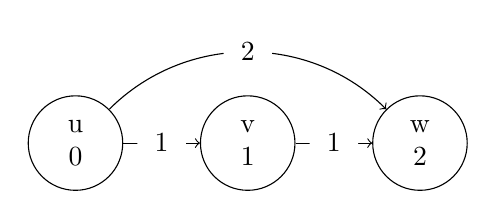
\begin{tikzpicture}[scale=1.75]
    \node[circle, draw, minimum size=1.2cm, inner sep=0pt , align=center] at (0*1.25, 0)  (u)    {u\\0};
    \node[circle, draw, minimum size=1.2cm, inner sep=0pt , align=center] at (1*1.25, 0)  (v)    {v\\1};
    \node[circle, draw, minimum size=1.2cm, inner sep=0pt , align=center] at (2*1.25, 0)  (w)    {w\\2};

    \draw[->]  (u) edge[bend left=45] node[circle, fill=white] {2} (w);
    \draw[->]  (u) edge node[circle, fill=white] {1} (v);
    \draw[->]  (v) edge node[circle, fill=white] {1} (w);
  \end{tikzpicture}
  \caption{Beispiel notwendiger Kanten im Upward-Graph}
  \label{fig:people:notwendige_kanten}
\end{figure}

\subsection{Kontraktion erfüllt diese Definition}

Bei der Knoten-Kontraktion des Knoten $v$ wird für den Pfad $(u, v, w)$ eine Abkürzung eingefügt, wenn dies der einzige kürzeste $u$-$w$-Pfad ist.
Ist dies der Fall, dann wurden die Knoten aller andern kürzesten Pfade zuvor bereits kontrahiert und haben daher ein niedrigeres Level.
Daher bilden diese Abkürzungen mitsamt den Kanten des ursprünglichen Graphen die Kantenmenge des Upward- und Downward-Graphen.
Wird die Kontraktionsbedingung abgeschwächt, so werden nicht notwendige, nicht optimale $(v, w)$ Kanten eingefügt, die dann einem nicht optimalen Pfad enstprechen auf dem $v$ und $w$ die beiden höchsten Level haben.
Daher entspricht ein durch Graphen-Kontraktion erzeugter Graph der neuen Definition.

\section{Contracted Graph Algorithmus}

Das Berechnen aller kürzesten Pfade zwischen zwei Knoten ist aufwändig, daher wird zum Berechnen eines so defineirten Contracted Graphens ein ähnlichen Trick angewendet, wie er bei der Knoten Kontraktion angewandt wird:
Wir fügen Kanten ein, sobald wir \emph{einen} optimalten $t$-$h$-Pfad gefunden haben, auf dem $h$ das größte und $t$ das zweitgrößte Level hat.
Dies ist hinreichend um die Bedingung zu erfüllen, fügt im Zweifel jedoch mehr Kanten als notwendig ein.

Um einen Upward Graphen zu berechnen, wird für jeden Knoten $t \in V$ eine angepasste Dijkstra Suche ausgeführt, bei der für jeden Knoten jeweils notiert wird, was größte Level auf dem Pfad zur Wurzel ist.
Dies Information kann mit der \emph{max-on-path} Funktion ${mop}$ abegrufen werden.
Ein Knoten $h \in V$, $h \neq t$ ist der Kopf eine Upward Graph Kante, für die gilt, dass ${mop}(h) = {vtl}(h)$ und ${mop}({pre}(h)) = {vtl}(t)$.
Das Gewicht der Kante kann der Dijkstra Suche entommen werden.
Die Suche kann abgebrochen werden, wenn nur noch Knoten für alle nicht-expandierten Knoten $h$ gilt dass ${mop}({pre}(h)) > {vtl}(h)$ ist.
\autoref{ch:fig:brute_force_suchbaum} zeigt dies für den Knoten $a$ im Beispielgraphen.
Die linke Zahl steht dabei für das Level des jeweiligen Knoten, die rechte Zahl für das größte Level auf dem Pfad zur Wurzel.

\begin{figure}[ht]
  \centering
  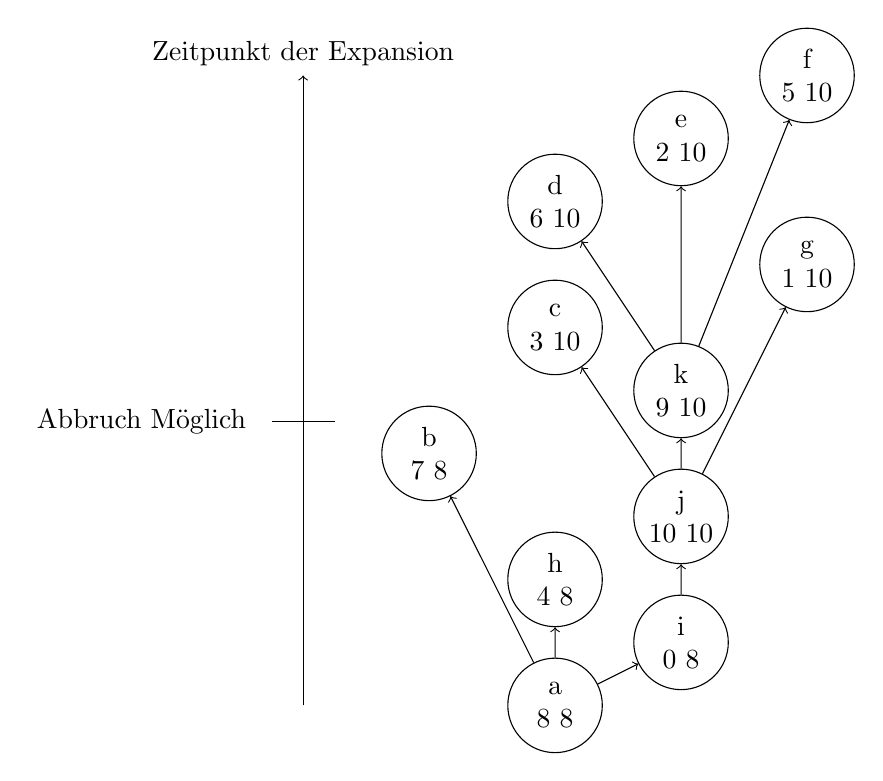
\begin{tikzpicture}[scale=0.8]
    % Nodes
    % a & b & c & d & e & f & g & h & i & j & k &
    % 8 & 7 & 3 & 6 & 2 & 5 & 1 & 4 & 0 & 10 & 9 &

    \node[circle, draw, minimum size=1.2cm, inner sep=0pt , align=center] at (2* 1, 0)  (a)    {a\\8 8};
    \node[circle, draw, minimum size=1.2cm, inner sep=0pt , align=center] at (2* 0, 4)  (b)    {b\\7 8};
    \node[circle, draw, minimum size=1.2cm, inner sep=0pt , align=center] at (2* 1, 6)  (c)    {c\\3 10};
    \node[circle, draw, minimum size=1.2cm, inner sep=0pt , align=center] at (2* 1, 8)  (d)    {d\\6 10};
    \node[circle, draw, minimum size=1.2cm, inner sep=0pt , align=center] at (2* 2, 9)  (e)    {e\\2 10};
    \node[circle, draw, minimum size=1.2cm, inner sep=0pt , align=center] at (2* 3, 10)  (f)    {f\\5 10};
    \node[circle, draw, minimum size=1.2cm, inner sep=0pt , align=center] at (2* 3, 7)  (g)    {g\\1 10};
    \node[circle, draw, minimum size=1.2cm, inner sep=0pt , align=center] at (2* 1, 2)  (h)    {h\\4 8};
    \node[circle, draw, minimum size=1.2cm, inner sep=0pt , align=center] at (2* 2, 1)  (i)    {i\\0 8};
    \node[circle, draw, minimum size=1.2cm, inner sep=0pt , align=center] at (2* 2, 3)  (j)    {j\\10 10};
    \node[circle, draw, minimum size=1.2cm, inner sep=0pt , align=center] at (2* 2, 5)  (k)    {k\\9 10};

    \draw[->]  (a) edge (b);
    \draw[->]  (a) edge (h);
    \draw[->]  (a) edge (i);
    \draw[->]  (j) edge (c);
    \draw[->]  (i) edge (j);
    \draw[->]  (k) edge (d);
    \draw[->]  (j) edge (k);
    \draw[->]  (k) edge (e);
    \draw[->]  (k) edge (f);
    \draw[->]  (j) edge (g);

    \draw[->] (-2, 0) -- (-2, 10) node[above] {Zeitpunkt der Expansion};

    \draw (-2.5, 4.5) -- (-1.5, 4.5) node[left=1cm] {Abbruch Möglich};

  \end{tikzpicture}
  \caption{Brute-Force Suche}
  \label{ch:fig:brute_force_suchbaum}
\end{figure}

Die Informtion des größten Levels auf dem Pfad zur Wurzel kann dabei beim Update eines Kontens übertragen werden, indem das Maximum des bisherigen größten Levels und das Level des upgedateten Knoten gebildet wird.
Die Abbruchbedingung kann durch die Verfolgung einer Menge an \emph{lebendigen Knoten} erzielt werden, sobald diese keine Knoten mehr entählt, kann die Suche abgebrochen werden.
Zu beginn ist nur der Startknoten lebendig, die Lebendigkeit wird jeweils an die Kinder vererbt.
Ein Knoten stirbt, nachdem er expandiert wurde oder wenn er den Kopf einer Kante bildet.
Gibt es keine lebendigen Knoten mehr, so kann die Suche abgebrochen werden.
In dem verwendeten Beispiel wäre dies etwa nach der Expansion von $b$ der Fall.
Die Berechung ist \emph{embarrassingly parallel}, da jeder Knoten für sich selbst Berechnet werden kann.
Der textuell beschriebene Algorithmus wird dann wie folgt formal definiert:

\begin{algorithm}[ht]
  \caption{Contracted Graph Brute Force Suchalgorithmus}
  \begin{algorithmic}[1]
    \Require Graph $G = (V, E)$, vertex-to-level Funktion ${vtl}$, Startknoten $s \in V$, Zielknoten $t \in V$
    \Ensure $E_s$
    \State // Initialisiere Distanz- und Vorgänger-Funktion
    \ForAll{$v \in V$}
    \State ${dist}(v) \leftarrow \infty$
    \State ${pre}(v) \leftarrow {none}$
    \EndFor

    \State
    \State // Initialisiere Suche
    \State ${dist}(s) \leftarrow 0$
    \State $Q\leftarrow \{ s \}$
    \State ${pre}(s) \leftarrow s$

    \State
    \State // Initialisiere max-on-path
    \State ${mop}(s) \leftarrow {vtl}(s)$
    \State $E_s \leftarrow \{ \}$
    \State ${alive} \leftarrow \{ s \}$

    \State
    \While{$Q \neq \emptyset \land {alive} \neq \emptyset$}
    \State $u \leftarrow{extract\_min}(Q)$\label{graphs:dijkstra:pop}

    \State
    \State // Beende frühzeitig wenn Zielknoten gefunden wurde
    \If {$u \neq s \land {mop}(u) = {vtl}(u)$}
    \State $E_s \leftarrow E_s \cup \{ (s, u, {dist}(u)) \}$
    \State ${alive} \leftarrow {alive} \setminus \{ s \}$
    \EndIf

    \State
    \State // Aktualisiere Nachbarn
    \ForAll{$(u, v, w) \in E$}
    \If {${dist}(u) + w < {dist}(v)$}
    \State ${dist}(v) \leftarrow {dist}(u) + w$
    \State ${pre}(u) \leftarrow v$
    \State $Q = Q \cup \{ v \}$
    \State
    \State // setze max\_level\_path
    \State ${mop}(v) \leftarrow \max({mop}(v), {vtl}(v))$
    \If {$u \in {alive}$}
    \State ${alive} \leftarrow {alive} \cup \{ s \}$
    \EndIf
    \EndIf
    \EndFor

    \State ${alive} \leftarrow {alive} \setminus \{ s \}$

    \EndWhile

    \State
    \State \Return $E_s$
  \end{algorithmic}
\end{algorithm}

\subsection{Abkürzung Problem}

Es liegt nahe als abgekürzten Knoten den Knoten mit dem dritthöchsten Level auszuwählen und sich darauf zu verlassen, dass die Suche von diesem Knoten aus die nächsen Abkürzung findet, da dies der Knoten-Kontraktion enstpricht.
Dies ist praktisch, da dann jeder Shortcut nur einmal erstellt werden muss, dafür muss jedoch gelten, dass die Vorwärtssuche für $s$-$t$ den gleichen Pfad findet wie die Rückwärtssuche (die Suche auf dem Transponierten Graphen) für $t$-$s$.
Wird als Graph eine Datenstruktur verwendet, welche die Nachbarn nicht in einer definierten Ordnung ausgibt (etwa ein Hashset), oder eine nicht stabile Prioritätswarteschlange verwendet, ist dies nicht garantiert.

\autoref{ch:fig:problem_shortcut} zeigt eine Situation, in der dies auftreten kann.
In $C$ wurde der Pfad $(a, e)$ gefunden, dess Abkürzungen jetzt ersetzt werden sollen.
Hierfür wird im ersten Schritt die für die Abkürzung $(a, e)$ der abgekürzte Knoten $d$ gefunden, dadurch ist der Pfad $(a, d, e)$.
Für den Knoten $a$ wird die Kante $(a, e)$ mit dem abgekürzten Knoten $d$ gefunden.
Wir verlassen uns darauf, dass die Suche von $d$ aus die Abkürzung $(d, a)$ mit dem Knoten $b$ findet, dies geschieht jedoch nicht, wenn von $d$ aus $a$ über $c$ erreicht wird.

\begin{figure}[h!]
  \centering

  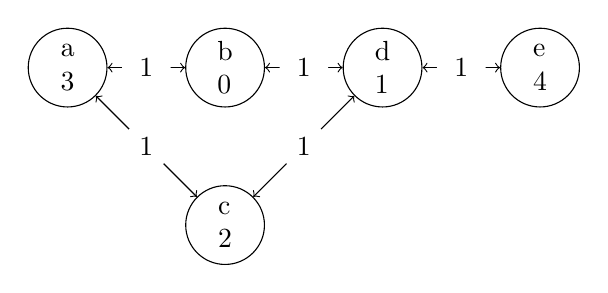
\begin{tikzpicture}
    % Nodes
    \node[circle, draw, minimum size=1cm, inner sep=0pt, align=left] at (2*0, 2*0)  (a)    {a\\3};
    \node[circle, draw, minimum size=1cm, inner sep=0pt, align=left] at (2*1, 2*0)  (b)    {b\\0};
    \node[circle, draw, minimum size=1cm, inner sep=0pt, align=left] at (2*1, 2*-1)  (c)    {c\\2};
    \node[circle, draw, minimum size=1cm, inner sep=0pt, align=left] at (2*2, 2*0)  (d)    {d\\1};
    \node[circle, draw, minimum size=1cm, inner sep=0pt, align=left] at (2*3, 2*0)  (e)    {e\\4};

    \draw[<->]  (a) edge node[circle, fill=white] {1} (b);
    \draw[<->]  (b) edge node[circle, fill=white] {1} (d);
    \draw[<->]  (d) edge node[circle, fill=white] {1} (e);

    \draw[<->]  (a) edge node[circle, fill=white] {1} (c);
    \draw[<->]  (c) edge node[circle, fill=white] {1} (d);
  \end{tikzpicture}
  \caption{Problem beim Shortcut erstellen}
  \label{ch:fig:problem_shortcut}
\end{figure}

Für dieses Problem gibt es zwei Lösungen:
Die Nachfolgenden Abkürzungen, welche benötigt werden, um eine Abkürzung vollständig zu entpacken werden für jede Abkürzung ebenfalls erstellt, dadurch werden viele Abkürzungen mehrfach erstellt, dies muss daher synchronisiert werden.
Alternativ kann die Prioritätswarteschlange modifiziert werden, indem es eine Totalordnung der Knoten gibt und diese bestimmt, in welcher Reihenfolge Knoten gleicher Distanz expandiert werden.

\section{Hub Labels Algorithmus}

Analog zur neuen Definition des Contracted-Graph lässt sich auch der Hub-Graph neu Definieren.
Die dafür verwendete Defintion der Forward-Label weicht nur leicht von der des Upward-Graphen ab.

\begin{definition}[Forward-Label]
  Sei $G = (V, E)$ und ${vtl}$ eine vertex-to-level Funktion dazu.
  Dann ist $L_f (t) \subset V \times \mathbb{R}$ ein Forward-Label für einen Knoten $t$ in $G$ wenn gilt:

  \begin{itemize}
    \item
      $L_f (t)$ enthält nur Einträge $(h, d)$ mit $h \in V$ und $d \in \mathbb{R}$, für die es einen $t$-$h$ Pfad der Länge $d \geq {spd}_G (t, g)$ gibt, so dass auf ihm $h$ das größte und $t$ das zweitgrößte Level hat.

    \item
      $L_f (t)$ enthält alle Einträge $(h, {spd}_G (t, h))$ mit $h \in V$, für die gilt, dass auf \emph{allen} $t$-$h$ Pfaden $h$ das größte und $t$ zweitgröste Level hat.
  \end{itemize}
\end{definition}

Hierbei ist ein Backward-Label ein Forward-Label das Transponierten Graphen $G^T$ .
Solche Label können wieder durch Merging aus einem Contracted-Graph erstellt worden durch eine Suche pro Knoten.
\todo{Algorithmus}
Die Suche pro Knoten erstellt dabei geprunte Label und kann kann auch dafür benutzt werden, die Qualität (durschnitliche Label Size) einer vertex-to-level Funktion anzugeben, ohne den kompletten Hub Graphen zu berechnen.
Hierfür würd für $n$ Knoten das Label berechnet und die größte des Labels angegeben.
Da sich dies leicht parallelisiern läst, könnte in einem zukünftigen Schritt durch Opmierungsalgorithmen die Label Size verkleinert werden.

\chapter{Ergebnisse}

Sofern nicht anders erwähnt wurden Systeme mit zwei Intel Xeon Gold 6230 Prozessoren mit einer Taktrate von 2.1 Ghz und 180GB RAM benutzt.
Die Ergebnisse wurden auf gleichen System, aber nicht auf demselben erzeugt.

\section{Untersuchung der Graphen}

Die bereitgestellten Graphen wurden vor ihrer Nutzung untersucht
Hierfür wurde zuerst die Verteilung der Knotengrade untersucht.
Dabei wurden die Histogramme in \autoref{ergebnisse:fig:degree_hist} erstellt.
Für jeden der Sichtbarkeitsgraphen gilt, dass mindestens 90\% aller Knoten einen Grad kleiner \num{2000} haben.

\begin{figure}[p]
  \begin{subfigure}[b]{0.5\textwidth}
    \resizebox{\textwidth}{!}{%
      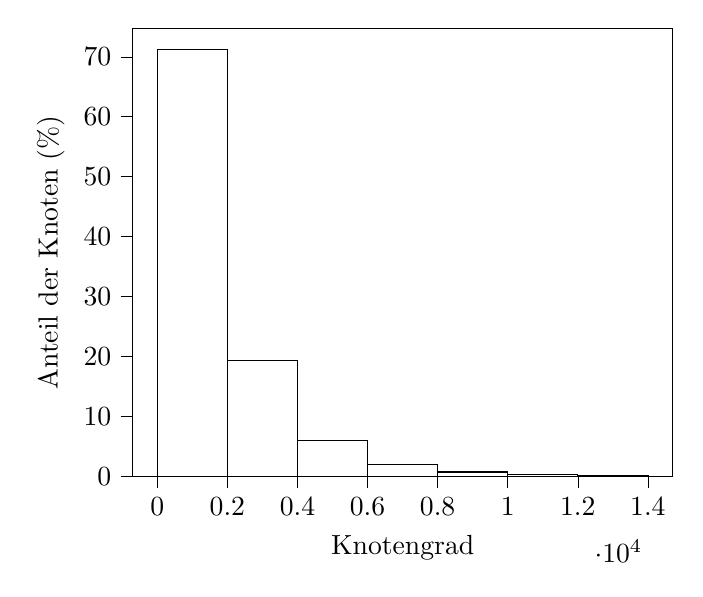
\begin{tikzpicture}
        \begin{axis}[
            tick align=outside,
            tick pos=left,
            xmin=-698, xmax=14702,
            xtick style={color=black},
            xtick distance=2000,
            ymin=0, ymax=0.747618384401001,
            ytick style={color=black},
            ytick={0,0.1,0.2,0.3,0.4,0.5,0.6,0.7,0.8},
            yticklabels={0,10,20,30,40,50,60,70,80},
            xlabel={Knotengrad},
            ylabel={Anteil der Knoten (\%)}
          ]
          \draw[] (axis cs:2,0) rectangle (axis cs:2002,0.712017508953334);
          \draw[] (axis cs:2002,0) rectangle (axis cs:4002,0.194220055711032);
          \draw[] (axis cs:4002,0) rectangle (axis cs:6002,0.0606247512935969);
          \draw[] (axis cs:6002,0) rectangle (axis cs:8002,0.0205382013530728);
          \draw[] (axis cs:8002,0) rectangle (axis cs:10002,0.00766514126545947);
          \draw[] (axis cs:10002,0) rectangle (axis cs:12002,0.00397930760049903);
          \draw[] (axis cs:12002,0) rectangle (axis cs:14002,0.000955033824119655);
        \end{axis}
      \end{tikzpicture}
    }
    \caption{aegaeis-vis}
  \end{subfigure}%
  \begin{subfigure}[b]{0.5\textwidth}
    \resizebox{\textwidth}{!}{%
      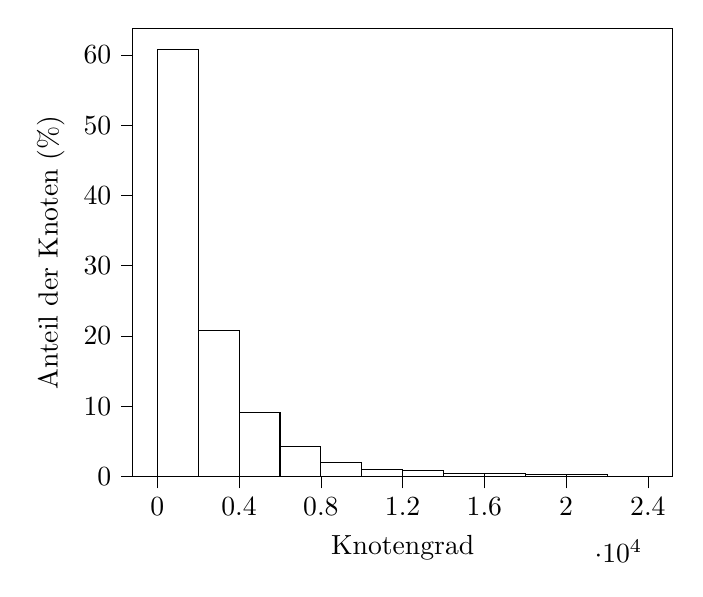
\begin{tikzpicture}
        \begin{axis}[
            tick align=outside,
            tick pos=left,
            xlabel={Knotengrad},
            xmin=-1198, xmax=25202,
            xtick distance=4000,
            xtick style={color=black},
            ylabel={Anteil der Knoten (\%)},
            ymin=0, ymax=0.637890337808629,
            ytick style={color=black},
            ytick={0,0.1,0.2,0.3,0.4,0.5,0.6,0.7},
            yticklabels={0,10,20,30,40,50,60,70}
          ]
          \draw[] (axis cs:2,0) rectangle (axis cs:2002,0.60751460743679);
          \draw[] (axis cs:2002,0) rectangle (axis cs:4002,0.207212784893063);
          \draw[] (axis cs:4002,0) rectangle (axis cs:6002,0.0905080679486225);
          \draw[] (axis cs:6002,0) rectangle (axis cs:8002,0.0423164235317719);
          \draw[] (axis cs:8002,0) rectangle (axis cs:10002,0.0196700589456533);
          \draw[] (axis cs:10002,0) rectangle (axis cs:12002,0.0103219440467273);
          \draw[] (axis cs:12002,0) rectangle (axis cs:14002,0.00818403436132265);
          \draw[] (axis cs:14002,0) rectangle (axis cs:16002,0.00425647177184629);
          \draw[] (axis cs:16002,0) rectangle (axis cs:18002,0.00420165357478464);
          \draw[] (axis cs:18002,0) rectangle (axis cs:20002,0.00342452501643997);
          \draw[] (axis cs:20002,0) rectangle (axis cs:22002,0.00236363167330556);
          \draw[] (axis cs:22002,0) rectangle (axis cs:24002,2.57967986172503e-05);
        \end{axis}
      \end{tikzpicture}
    }
    \caption{medi-vis}
  \end{subfigure}
  \par\bigskip
  \begin{subfigure}[b]{0.5\textwidth}
    \resizebox{\textwidth}{!}{%
      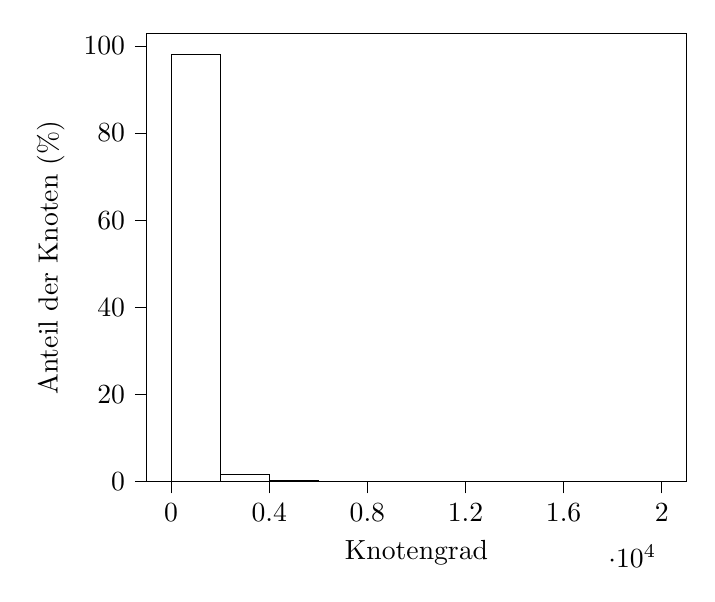
\begin{tikzpicture}
        \begin{axis}[
            tick align=outside,
            tick pos=left,
            xlabel={Knotengrad},
            ylabel={Anteil der Knoten (\%)},
            xmin=-998, xmax=21002,
            xtick style={color=black},
            y grid style={darkgray176},
            xtick distance=4000,
            ymin=0, ymax=1.02857224104146,
            ytick style={color=black},
            ytick={0,0.2,0.4,0.6,0.8,1,1.2},
            yticklabels={0,20,40,60,80,100,120}
          ]
          \draw[] (axis cs:2,0) rectangle (axis cs:2002,0.979592610515676);
          \draw[] (axis cs:2002,0) rectangle (axis cs:4002,0.0169022235303201);
          \draw[] (axis cs:4002,0) rectangle (axis cs:6002,0.00222602483448042);
          \draw[] (axis cs:6002,0) rectangle (axis cs:8002,0.000968834654540784);
          \draw[] (axis cs:8002,0) rectangle (axis cs:10002,0.000297335455255565);
          \draw[] (axis cs:10002,0) rectangle (axis cs:12002,3.99107993631631e-06);
          \draw[] (axis cs:12002,0) rectangle (axis cs:14002,0);
          \draw[] (axis cs:14002,0) rectangle (axis cs:16002,9.97769984079078e-07);
          \draw[] (axis cs:16002,0) rectangle (axis cs:18002,3.99107993642733e-06);
          \draw[] (axis cs:18002,0) rectangle (axis cs:20002,3.99107993631631e-06);
        \end{axis}

      \end{tikzpicture}
    }
    \caption{pata-vis}
  \end{subfigure}
  \caption{Verteilung der Kantengrade}
  \label{ergebnisse:fig:degree_hist}
\end{figure}

Wie diskutiert ist die Summe der quadratischen Knotengrade ein Indikator für die Performanz der Kontraktion.
Diese sind in \autoref{table:sum_quad_degree} sichtbar.
Obwohl pata die meisten Knoten hat, ist die summe der Quadrate am kleinsten.

Dann naive Rechnung: Knoten-Differenz soll in einem Tag stattfinden, 40 Kerne.
Wieviel Zeit pro Paar?

\begin{table}[ht]
  \centering
  \begin{tabular}{
      l % Graph
      S[table-format = 13.0] % Zeit
      S[table-format = 3.1] % Zeit pro Paars
    }
    \toprule
    {Graph}            & {$\sum_{v \in V} (\text{Grad}(v))^2$} & {Zeit pro paar in us}                       \\ \midrule
    aegaeis-visibility & 1153579966074                         & \fpeval{(10e6)*40*(24*60*60)/1153579966074} \\
    medi-visibility    & 4667069733248                         & \fpeval{(10e6)*40*(24*60*60)/4667069733248} \\
    pata-visibility    & 426189267238                          & \fpeval{(10e6)*40*(24*60*60)/426189267238}  \\ \bottomrule
  \end{tabular}
  \caption{Summe quadratische Knotengrade}
  \label{table:sum_quad_degree}
\end{table}

\todo{Boxplot für alle Hops über 80 und Triangulierung}

% aegaeis
% 75.6658\% korrekt
% 0.40990444596118253 average
%
% %WARUM MEDI, PATA nicht so korrekt?
% \todo{STIMMEN ZAHLEN?}
%
% medi
% 0.39110000000000006\% korrekt
% 0.9727677753480117 average
%
% pata
% 0.068\% korrekt
% 0.6179520250326755 average

\subsection{Dijkstra}

Für die Berechnung des Speedups der in dieser Arbeit angewandeten Methoden wurden für jeden Graph \num{1000} sequentielle $s$-$t$ Dijkstra-Suchen asugeführt und die durschnittliche Laufzeit ermittelt.
Die durschnittliche Laufzeiten für das Finden und erstellen des kürzesten Pfad sind in Tabelle \ref{fig:ergebnisse:dijkstra} dargestellt.
Es ist ersichtlich, dass die Sichtbarkeitsgraphen im Vergleich zu ihren Triangulierungen deutlich höhere Laufzeiten haben.

Zusätzlich zur durschnitlichen Laufzeit wurde die die Durschnitswerte der Hop-Länge, des Dijsktra-Rank und der Queue pops ermittelt, um ein Verständnis für die Laufzeiten zu erlangen.
Es zeigte sich, dass die durschnittliche Hop-Länge der Sichtbarkeitsgraphen deutlich signifikant kürzer ist, als die der Triangulierungen.
Obwohl die Sichtbarkeitsgraphen eine niedriger Anzahl an Knoten haben, ist die durschnitliche Anzahl der Queue pops größer.
Dies legt Nahe, dass die verwendung einer Warteschlange, welche eine \emph{Drecrease-Key} Funktion anbietet, die Geschwindigkeit der Dijkstra Suche erhöhen würde.

\begin{table}[h!]
  \centering
  \begin{tabular}{
      l % Graph
      S[table-format = 4.1] % Zeit
      S[table-format = 3.0] % hop-länge
      S[table-format = 7.0] % rank
      S[table-format = 7.0] % queue pops
    }
    \toprule
    {Graph}            & {$\varnothing$ $t({spd})$} & {$\varnothing$  Hop-Länge} & {$\varnothing$ Dijkstra Rank} & {$\varnothing$ Queue pops} \\
                       & {(\si{\ms})}               &                            &                               &                            \\
    \midrule
    aegaeis-graph      & 60.281198                  & 215.7201                   & 260447.36                     & 325845.56                  \\
    aegaeis-visibility & 630.434928                 & 16.311                     & 98650.82                      & 517346.63                  \\
    medi-graph         & 87.08376                   & 340.445                    & 394855.78                     & 494553.97                  \\
    medi-visibility    & 1279.67479                 & 23.6149                    & 154092.42                     & 959206.4                   \\
    pata-graph         & 265.825771                 & 883.979                    & 1120841.9                     & 1387047.8                  \\
    pata-visibility    & 1017.695977                & 63.817                     & 498570.2                      & 2429689.8                  \\ \bottomrule
  \end{tabular}
  \caption{Durschnitliche Kennwerte der Dijkstra Suchen (über \num{10000} Suchen)}
  \label{fig:ergebnisse:dijkstra}
\end{table}

\section{Graphen-Kontraktion}

Ausgangspunkt der Analyzse, ob sich die in dieser Arbeit bearbeiteten Sichtbarkeitsgraphen kontrahieren lassen, war die Anwendung der klassischen Graphen-Kontraktion mit Witness-Suche, wobei ein für diese Arbeit entwickeltes Programm genutzt wurde.
Die Reihenfolge der Kontrraktion wurde dabei durch die Kanten-Differenz mit Lazy-Popping bestimmt.
Für die triangulierten Graphen war es möglich einen Contracted-Graphen zu erstellen, die Bearbeitung der Sichtbarkeitsgraphen wurde nach drei Tagen abgebrochen, wobei in dieser Zeit noch nicht alle initalen Kanten-Differenzen berechnet wurden.
Die Ergebnisse der trianguleirten Graphen sind in Tabelle \autoref{fig:ergebnisse:ch_graph_kontraktion_triangulierungen} zu sehen.

\begin{table}[h!]
  \centering
  \begin{tabular}{
      l % Graph
      r % Erstellung
      S[table-format = 1.2] % Abkürzungen/Katen
      S[table-format = 9.0] % average time spd
      S[table-format = 4.0] % speedup
    }
    \toprule
    {Graph}       & {Erstellung} & {$\frac{\text{Abkürzungen} (C)}{\text{Kanten} (G)}$} & {$\varnothing$ $t({spd})$} & {Speedup}                          \\
    {}            & {(min)}      & {}                                                   & {(\si{\us})}               & {}                                 \\
    \midrule
    aegaeis-graph & 2m 22s       & \fpeval{3047836/2795322}                             & 313.966                    & \fpeval{(60.281198*1000)/313.966}  \\
    medi-graph    & 3m 17s       & \fpeval{4535136/4223566}                             & 304.089                    & \fpeval{(87.08376*1000)/304.089}   \\
    pata-graph    & 9m 54s       & \fpeval{14187336/11632900}                           & 435.552                    & \fpeval{(265.825771*1000)/435.552} \\  \bottomrule
  \end{tabular}
  \caption{CH Graphen-Kontraktion}
  \label{fig:ergebnisse:ch_graph_kontraktion_triangulierungen}
\end{table}

Bassierend auf den Contracted-Graphen wurde jeweils ein Hub-Graph berechnet, die Ergebnisse hierfür sind in \autoref{fig:ergebnisse:hl_graph_kontraktion_triangulierungen} zu sehen.

\begin{table}[h!]
  \centering
  \begin{tabular}{
      l % Graph
      r % Erstellung
      S[table-format = 3.0] % label
      S[table-format = 3.2] % average time spd
      S[table-format = 6.] % speedup
    }
    \toprule
    {Graph}       & {Erstellung}     & {$\varnothing$ $\abs{\text{Label}}$} & {$\varnothing$ $t({spd})$} & {Speedup}                        \\
    {}            & {}               & {}                                   & {(\si{\us})}               & {}                               \\
    \midrule
    aegaeis-graph & 7m 11s           & 141.4722365640974                    & 2.334                      & \fpeval{(60.281198*1000)/2.334}  \\
    medi-graph    & 9m \phantom{0}1s & 115.88322360565405                   & 1.893                      & \fpeval{(87.08376*1000)/1.893}   \\
    pata-graph    & 29m 45s          & 133.48887779929734                   & 2.415                      & \fpeval{(265.825771*1000)/2.415} \\
    \bottomrule
  \end{tabular}
  \caption{HL Graphen-Kontraktion}
  \label{fig:ergebnisse:hl_graph_kontraktion_triangulierungen}
\end{table}

Als zusätzlicher Anhaltspunkt um die Qualität der erzeugten Contracted-Graphen zu beurteilen wurde ein externes Programm benutzt, um ebenfalls Contracted-Graphen zu erzeugen.
Die Ergebnisse hierfür sind in \autoref{fig:ergebnisse:fmi_ch_graph_kontraktion_triangulierungen} aufgelistet.
Da dieses Programm ein anders Format zur Speicherung benutz, wurden die Anfrage-Zeiten nicht erhoben.
Dieses Programm kontrahiert mehrere Knoten gleichzeitig, indem es \emph{Unabhänige Teilmengen} von Knoten findet, und kann daher besser parallel arbeiten, durch den hohen Grad der Sichtbarkeitsgraphen ist jedoch anzunehmen, dass es nur wenige, kleine unabhängige Teilmengen gibt.
Auch dieses Programm hat nach drei Tagen Laufzeit auf den Sichtbarkeitsgraphen keine Ergebnisse produziert.


\begin{table}[h!]
  \centering
  \begin{tabular}{
      l % Graph
      r % Erstellung
      S[table-format = 1.2] % Abkürzungen/Katen
      S[table-format = 9.0] % average time spd
      S[table-format = 4.0] % speedup
    }
    \toprule
    {Graph}       & {Erstellung} & {$\frac{\text{Abkürzungen} (C)}{\text{Kanten} (G)}$} \\
    {}            & {(min)}      & {}                                                   \\
    \midrule
    aegaeis-graph & 22s          & \fpeval{(5446922-(2795322/2))/2795322}               \\
    medi-graph    & 34s          & \fpeval{(8156314-(4223566/2))/4223566}               \\
    pata-graph    & 1m 48s       & \fpeval{(23557322-(11632900/2))/11632900}            \\  \bottomrule
  \end{tabular}
  \caption{FMI CH Graphen-Kontraktion}
  \label{fig:ergebnisse:fmi_ch_graph_kontraktion_triangulierungen}
\end{table}

\subsection{Kontraktion mit oberer Schranke}

\todo{Alles :D}


\begin{figure}[p]% Die Daten in den .csv Dateien sind gelippt auf 100. pgf hat Probleme mit zu großen Zahlen.
  \begin{subfigure}[b]{0.5\textwidth}
    \resizebox{\textwidth}{!}{%
      \begin{tikzpicture}
        \begin{axis}[
            ymax=6,
            xlabel={Hop-Länge},
            ylabel={Fehler (\%)},
            legend style={at={(1,0.475)},anchor=east, nodes={scale=0.8, transform shape}}
          ]
          \addplot+[mark repeat=9] table [x=hops, y=simple_graph_upper_bound, col sep=comma] {data/bounds/aegaeis.csv};
          \addlegendentry{$\triangle$};

          \addplot+[mark repeat=9] table [x=hops, y=10, col sep=comma] {data/bounds/aegaeis.csv};
          \addlegendentry{10 Hubs};

          \addplot+[mark repeat=9] table [x=hops, y=20, col sep=comma] {data/bounds/aegaeis.csv};
          \addlegendentry{20 Hubs};

          \addplot+[mark repeat=9] table [x=hops, y=40, col sep=comma] {data/bounds/aegaeis.csv};
          \addlegendentry{40 Hubs};

          \addplot+[mark repeat=9] table [x=hops, y=80, col sep=comma] {data/bounds/aegaeis.csv};
          \addlegendentry{80 Hubs};

          \addplot+[mark repeat=9] table [x=hops, y=min_80_simple, col sep=comma] {data/bounds/aegaeis.csv};
          \addlegendentry{$\triangle$, 80 Hubs};
        \end{axis}
      \end{tikzpicture}
    }
    \caption{aegaeis-vis}
  \end{subfigure}%
  \begin{subfigure}[b]{0.5\textwidth}
    \resizebox{\textwidth}{!}{%
      \begin{tikzpicture}
        \begin{axis}[
            ymax=6,
            xlabel={Hop-Länge},
            ylabel={Fehler (\%)},
            legend style={at={(1,0.475)},anchor=east, nodes={scale=0.8, transform shape}}
          ]
          \addplot+[mark repeat=12] table [x=hops, y=simple_graph_upper_bound, col sep=comma] {data/bounds/medi.csv};
          \addlegendentry{$\triangle$};

          \addplot+[mark repeat=12] table [x=hops, y=10, col sep=comma] {data/bounds/medi.csv};
          \addlegendentry{10 Hubs};

          \addplot+[mark repeat=12] table [x=hops, y=20, col sep=comma] {data/bounds/medi.csv};
          \addlegendentry{20 Hubs};

          \addplot+[mark repeat=12] table [x=hops, y=40, col sep=comma] {data/bounds/medi.csv};
          \addlegendentry{40 Hubs};

          \addplot+[mark repeat=12] table [x=hops, y=80, col sep=comma] {data/bounds/medi.csv};
          \addlegendentry{80 Hubs};

          \addplot+[mark repeat=12] table [x=hops, y=min_80_simple, col sep=comma] {data/bounds/medi.csv};
          \addlegendentry{$\triangle$, 80 Hubs};
        \end{axis}
      \end{tikzpicture}
    }
    \caption{medi-vis}
  \end{subfigure}
  \par\bigskip
  \begin{subfigure}[b]{0.5\textwidth}
    \resizebox{\textwidth}{!}{%
      \begin{tikzpicture}
        \begin{axis}[
            ymax=6,
            xlabel={Hop-Länge},
            ylabel={Fehler (\%)},
            legend style={at={(1,0.475)},anchor=east, nodes={scale=0.8, transform shape}}
          ]
          \addplot+[mark repeat=25] table [x=hops, y=simple_graph_upper_bound, col sep=comma] {data/bounds/pata.csv};
          \addlegendentry{$\triangle$};

          \addplot+[mark repeat=25] table [x=hops, y=10, col sep=comma] {data/bounds/pata.csv};
          \addlegendentry{10 Hubs};

          \addplot+[mark repeat=25] table [x=hops, y=20, col sep=comma] {data/bounds/pata.csv};
          \addlegendentry{20 Hubs};

          \addplot+[mark repeat=25] table [x=hops, y=40, col sep=comma] {data/bounds/pata.csv};
          \addlegendentry{40 Hubs};

          \addplot+[mark repeat=25] table [x=hops, y=80, col sep=comma] {data/bounds/pata.csv};
          \addlegendentry{80 Hubs};

          \addplot+[mark repeat=25] table [x=hops, y=min_80_simple, col sep=comma] {data/bounds/pata.csv};
          \addlegendentry{$\triangle$, 80 Hubs};
        \end{axis}
      \end{tikzpicture}
    }
    \caption{pata}
  \end{subfigure}
  \caption{Fehler der oberen Schranken}
\end{figure}


\section{PEOPLE}

Die in \autoref{chapter:peopel} vorgestellte Methode zur Berechnung von Contracted und Hub Graphen lies sie auch die Sichtbarkeitsgraphen und ihre Triangulierungen anwenden.

\subsection{Contracted Graph}

Die in \autoref{chapter:peopel} vorgestellte Methode zur Berechnung eines Contracted Graphens lies sich auf alle Graphen anwenden.
Die erzielten Werte der ERstellung sind in \autoref{table:ergebnisse:people_ch_erstellung} gesammelt.

Der Speedup ist in \autoref{table:ergebnisse:people_ch_speedup} zusammgenfasst.
Der Speedup der Trianuglierten Graphen ist deutlich kleiner, als der mit CH Witness, jedoch eine größenordnung schneller.
Der Speedup der Sichtbarkeitsgraphen ist kleines als eine Größenordnung.
Das sollte noch erkundet werden, warum.

pata hat trotzem mehr Speedup, weil von der Struktur her schon fast ein Straßengraph

\begin{table}[h!]
  \centering
  \begin{tabular}{
      l % Graph
      S[table-format = 4.0] % Erstellung
      S[table-format = 1.2] % Abkürzungen/Katen
      S[table-format = 3.2] % average time spd
      S[table-format = 3.2] % speedup
    }
    \toprule
    {Graph}            & {Erstellung} & {$\frac{\text{Abkürzungen} (C)}{\text{Kanten} (G)}$} & {$\varnothing$ $t({spd})$} & {Speedup}                      \\
    {}                 & {}           & {}                                                   & {(\si{\ms})}               & {}                             \\ \midrule
    aegaeis-graph      &              & \fpeval{12443056/2795322}                            & 2.290886                   & \fpeval{60.281198/2.290886}    \\
    aegaeis-visibility &              & \fpeval{214987558/310231834}                         & 408.948758                 & \fpeval{630.434928/408.948758} \\
    medi-graph         &              & \fpeval{20003908/4223566}                            & 3.38788                    & \fpeval{87.08376/3.38788}      \\
    medi-visibility    &              & \fpeval{468641256/730772544}                         & 832.555567                 & \fpeval{1279.67479/832.555567} \\
    pata-graph         &              & \fpeval{70624466/11632900}                           & 10.16729                   & \fpeval{265.825771/10.16729}   \\
    pata-visibility    &              & \fpeval{613324174/315653758}                         &                            & \fpeval{1017.695977/1}         \\  \bottomrule
  \end{tabular}
  \caption{Speedup der mit PEOPLE erstellten Contracted Graphen}
  \label{table:ergebnisse:people_ch_speedup}
\end{table}

\subsection{Hub Graph}

\subsubsection{Bootstraping HL}

Das Merging war deutlicht teruer als erwartet.
Dies ist dadurch zu erklären, dass für jeden Knoten die Anzahl der ausgehenden Contrated Graph Knoten viele Labels gemerged werden, welche durschnitlich sehr groß sind.
Das Mergen lässt sich aber gut parallisieren, durch eine Fold Operation, bei der jeder Thread für sich eine Menge an Labels merged.

\begin{table}[ht]
  \centering
  \begin{tabular}{ % DIREKT
      l % Graph
      S[table-format = 4.0] % creation zeit
      S[table-format = 4.1] % average time
    }
    \toprule
    {Graph}            & {Erstellung}       & {$\varnothing$ Label Größe} \\
    {}                 & {(min)}            & {}                          \\ \midrule
    aegaeis-graph      & 86.55              & 225.21998319619112          \\
    aegaeis-visibility & 357.9166666666667  & 2447.866444488659           \\
    medi-graph         & 191.06666666666666 & 262.34248736183486          \\
    medi-visibility    & 1317.85            & 3528.6126965393596          \\
    pata-graph         & 1706.5333333333333 & 451.8001829187458           \\
    pata-visibility    & 2657.5             & 1823.062327697596           \\  \bottomrule
  \end{tabular}
  \caption{Erstellung von Hub Graphen mit PEOPLE}
\end{table}


\begin{table}[h!]
  \centering
  \begin{tabular}{
      l % Graph
      r % Erstellung
      S[table-format = 3.1] % label
      S[table-format = 3.2] % average time spd
      S[table-format = 6.] % speedup
    }
    \toprule
    {Graph}       & {Erstellung}     & {$\varnothing$ $\abs{\text{Label}}$} & {$\varnothing$ $t({spd})$} & {Speedup}                        \\
    {}            & {}               & {}                                   & {(\si{\us})}               & {}                               \\
    \midrule
    aegaeis-graph & 7m 11s           & 141.4722365640974                    & 2.334                      & \fpeval{(60.281198*1000)/2.334}  \\
    medi-graph    & 9m \phantom{0}1s & 115.88322360565405                   & 1.893                      & \fpeval{(87.08376*1000)/1.893}   \\
    pata-graph    & 29m 45s          & 133.48887779929734                   & 2.415                      & \fpeval{(265.825771*1000)/2.415} \\
    \bottomrule
  \end{tabular}
  \caption{Erstellung von Hub Graphen mit PEOPLE}
\end{table}

\subsubsection{Direkt HL}

Das Anwenden des des Algorithmus zur Berechnung des Hub GRaphens hat gut funktioniert.
\todo{DIE LABELS SIND MINIMAL UNTERSCHIEDLICH GROß}

\begin{table}[h!]
  \centering
  \begin{tabular}{
      l % Graph
      r % Erstellung
      S[table-format = 3.1] % label
      S[table-format = 3.2] % average time spd
      S[table-format = 6.] % speedup
    }
    \toprule
    {Graph}            & {Erstellung} & {$\varnothing$ $\abs{\text{Label}}$} & {$\varnothing$ $t({spd})$} & {Speedup}  \\
    {}                 & {}           & {}                                   & {(\si{\us})}               & {}         \\
    \midrule1
    aegaeis-graph      &              & 225.18963155458096                   &                            & \fpeval{1} \\
    aegaeis-visibility &              & 2446.9511241543973                   &                            & \fpeval{1} \\
    medi-graph         &              & 262.32183266591755                   &                            & \fpeval{1} \\
    medi-visibility    &              & 3527.5645951837378                   &                            & \fpeval{1} \\
    pata-graph         &              & 451.71017734369667                   &                            & \fpeval{1} \\
    pata-visibility    &              & 1822.0561604813242                   &                            & \fpeval{1} \\
    \bottomrule
  \end{tabular}
  \caption{Erstellung von Hub Graphen durch Merging der mit PEOPLE erzeugen Contracted Graphen}
\end{table}

\subsubsection{Vergleich}

Für die Sichtbarkeitsgraphen ist es effizienter direkt die HL zu berechen.
Für die Triangulierten gRaphen ist es effizietner zuerst die  Contrated Graphen zu berechen.

\begin{table}[ht]
  \centering
  \begin{tabular}{ %VERGLEICH
      l % Graph
      S[table-format = 4.0] % creation zeit
      S[table-format = 4.0] % average time
    }
    \toprule
    {Graph}            & {CH \& Merging}               & {HL DIREKT}                  \\
    {}                 & {(min)}                       & {(min)}                      \\ \midrule
    aegaeis-graph      & \bfseries 32.5                & 86.55                        \\
    aegaeis-visibility & 809.3                         & \bfseries  357.9166666666667 \\
    medi-graph         & \bfseries  57.96666666666667  & 191.06666666666666           \\
    medi-visibility    & 2591.15                       & \bfseries  1317.85           \\
    pata-graph         & \bfseries  424.65000000000003 & 1706.5333333333333           \\
    pata-visibility    & 3532.366666666667             & \bfseries 2657.5             \\  \bottomrule
  \end{tabular}
  \caption{HL  merged}
\end{table}

\subsection{Vertex-to-level Vergeleich}

\begin{table}[]
  \centering
  \begin{tabular}{l
      S[table-format = 6.0] % random
      S[table-format = 6.0] % random
      S[table-format = 6.0] % random
      S[table-format = 6.0] % random
      S[table-format = 6.0] % random
      S[table-format = 6.0] % random
    }
    \toprule
    Graph              & \multicolumn{3}{c}{Hitting-Set}          & {$\triangle$}     & {Zufällig} & {Grad}   \\ \cline{2-4}
                       & {Zufällig} & {Hits}            & {Grad}  &                   &            &          \\
    \midrule
    aegaeis-visibility & 1747.03    & \bfseries 1420.17 & 1582.00 & 1473.27           & 17811.58   & 7420.85  \\
    medi-visibility    & 2487.06    & 2002.87           & 2422.12 & \bfseries 1930.65 & 18700.13   & 12862.80 \\
    pata-visibility    & 1100.42    & \bfseries 478.80  & 806.95  & 552.90            & 23690.52   & 10174.37 \\
    \bottomrule
  \end{tabular}
\end{table}


\printbibliography

\end{document}